% =============================================================================
% Capitulo 5 - Pruebas y resultados
% =============================================================================
\chapter{Pruebas y resultados}
\label{cap:pruebas_resultados}

% =============================================================================
\section{Preguntas de investigación}
\label{sec:preguntas_investigacion}

El sistema desarrollado en este trabajo comprende dos etapas encadenadas: una primera etapa de detección de ráfagas FHSS mediante YOLOv8, y una segunda etapa de clasificación de modelos de dron mediante ResNet18. Este capítulo valida ambas etapas respondiendo a cuatro preguntas de investigación, presentadas en el orden en que surgieron a lo largo del trabajo:

\begin{enumerate}
  \item \textbf{P1 ---} ¿Puede un clasificador global distinguir espectrogramas con señal de dron de los que contienen únicamente interferencia?
  \item \textbf{P2 ---} ¿Puede un detector de objetos localizar y separar morfológicamente las ráfagas FHSS de OcuSync de las interferencias presentes en la banda de \SI{2.4}{\giga\hertz}?
  \item \textbf{P3 ---} ¿Permiten las detecciones anteriores confirmar operativamente la presencia de un dron en una ventana temporal de \SI{0.1}{\second}?
  \item \textbf{P4 ---} ¿Puede el sistema identificar el modelo concreto de dron y discrimina su decisión por la morfología espectro-temporal de las ráfagas o por el nivel medio de potencia?
\end{enumerate}

Las dos primeras articulan la evolución metodológica del trabajo: la primera establece que la firma OcuSync es aprendible pero motiva el paso a un detector de objetos, y la segunda evalúa ese detector. Las dos últimas cuantifican el rendimiento operativo y la solidez del sistema definitivo.

Para cada pregunta se expone la descripción del experimento, los resultados obtenidos y una discusión de los mismos. Las métricas específicas de cada bloque se definen en el apartado correspondiente, junto con el experimento que las emplea.

% =============================================================================
\section{Conjunto de datos de evaluación}
\label{sec:dataset_evaluacion}

Las preguntas P1, P2 y P3 se responden sobre el dataset~v3 cuya captura, composición y generación de espectrogramas se describen en el \cref{cap:implementacion}. El conjunto consta de \num{3150}~espectrogramas de \num{1024}×\num{576}~píxeles, particionados por captura completa para evitar fuga de información entre particiones (véase \cref{subsec:diseno_dataset}). El conjunto de prueba comprende \num{600}~imágenes con balance exacto de \num{300}~\emph{drone} y \num{300}~\emph{interference}, y es el que se emplea para reportar todos los resultados de test de este capítulo. La pregunta~P4 emplea adicionalmente un conjunto de capturas de campo abierto con drones reales, descrito al inicio de la \cref{sec:bloque_clasificacion}.

% =============================================================================

% =============================================================================
% P1 --- version revisada: GradCAM como evidencia de que la clasificacion
% global NO se apoya en la morfologia de las rafagas.
% Sustituye integramente la seccion P1 del capitulo 5.
% Figuras nuevas: resnet18_gradcam_drone.png y resnet18_gradcam_interference.png
% (versiones de dos columnas: Entrada | GradCAM de la clase verdadera).
% =============================================================================

\section{P1 --- ¿Es reconocible la firma OcuSync mediante clasificación global?}
\label{sec:bloque_resnet_detector}

\subsection{Planteamiento del experimento}
\label{sec:p1_planteamiento}

La primera aproximación al problema consiste en entrenar un clasificador binario ResNet18 sobre el espectrograma completo para asignar la etiqueta \emph{drone} o \emph{interference} a cada imagen. Esta formulación evita la complejidad del etiquetado regional: basta con la etiqueta de la captura de la que procede cada espectrograma.

Se parte de una ResNet18 preentrenada en ImageNet, congelando las primeras tres capas y sustituyendo la cabeza de clasificación original por una capa \texttt{Linear(512,~2)}. El modelo se entrena durante \num{20}~épocas con el optimizador AdamW (tasa de aprendizaje \num{1e-4}, \emph{weight decay} \num{1e-4}), planificador \texttt{CosineAnnealingLR} y tamaño de lote \num{32}. Se aplica la normalización frecuencial \texttt{FrequencyNormalize} y la semilla se fija en 42.

\subsection{Resultados}
\label{sec:p1_resultados}

La \cref{fig:resnet18_binary_curvas} muestra la evolución de la pérdida y el F1~macro en entrenamiento y validación a lo largo de las veinte épocas.

\begin{figure}[htbp]
    \centering
    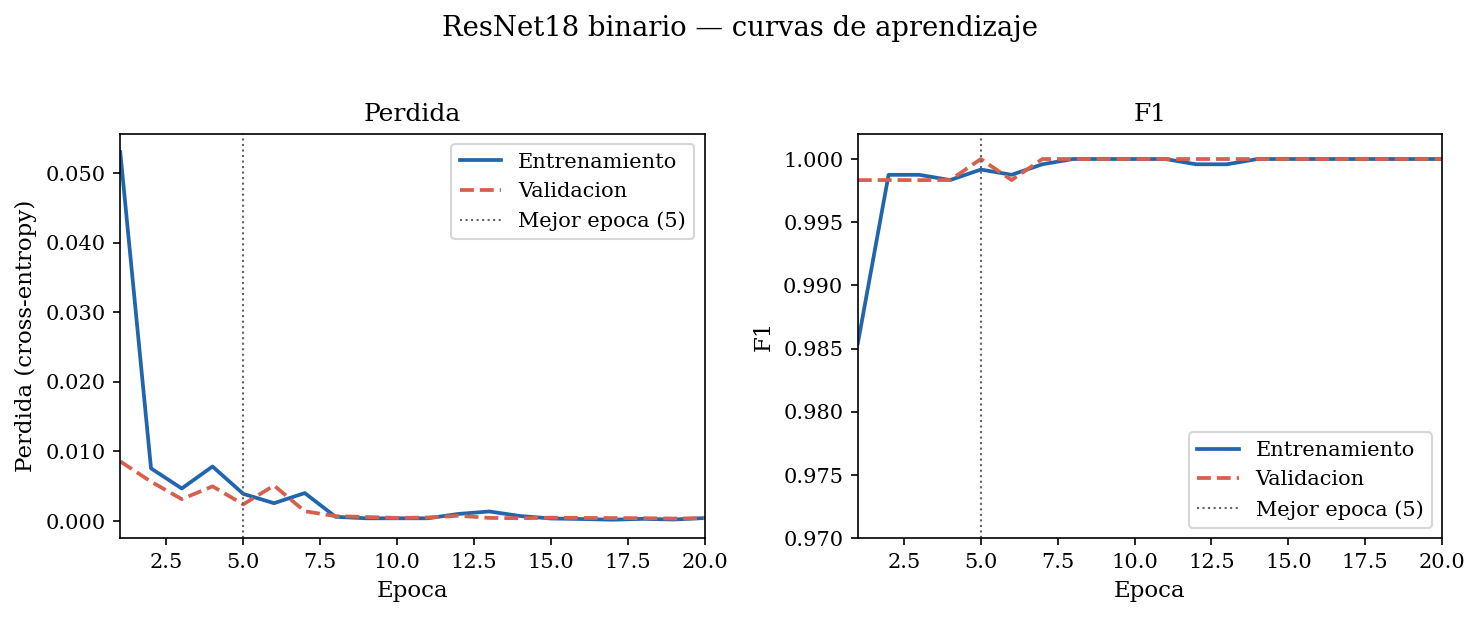
\includegraphics[width=0.85\textwidth]{figuras/resultados/resnet18_binary_curvas.png}
    \caption{Evolución de la pérdida y el F1~macro en entrenamiento y validación del clasificador ResNet18 binario a lo largo de las veinte épocas. La convergencia es extremadamente rápida: en menos de cinco épocas el F1 de validación alcanza \num{1,000}. La pérdida de validación se sitúa consistentemente por debajo de la de entrenamiento, lo que es habitual cuando el \emph{dropout} penaliza la pasada de entrenamiento pero no la de validación. No se observa sobreajuste en las curvas.}
    \label{fig:resnet18_binary_curvas}
\end{figure}

El modelo converge en menos de cinco épocas. La \cref{tab:p1_curva} detalla los valores de las primeras ocho épocas. En las épocas~1 a~4 el clasificador comete exactamente un error sobre las \num{450}~muestras de validación (F1~val = 0,998), que corresponde a una única muestra de interferencia con ráfagas Bluetooth morfológicamente próximas a OcuSync. Este error desaparece en la época~5, a partir de la cual el F1~de validación alcanza \num{1,000} con oscilaciones mínimas (una vuelta a \num{0,998} en la época~6, seguida de estabilización en \num{1,000} a partir de la época~7).

\begin{table}[htbp]
\centering
\caption{Pérdida y F1~macro durante las primeras ocho épocas del clasificador ResNet18 binario.}
\label{tab:p1_curva}
\begin{tabular}{ccccc}
\toprule
\textbf{Época} & \textbf{Loss train} & \textbf{F1 train} & \textbf{Loss val} & \textbf{F1 val} \\
\midrule
1 & 0,0530 & 0,985 & 0,0085 & 0,998 \\
2 & 0,0075 & 0,999 & 0,0056 & 0,998 \\
3 & 0,0046 & 0,999 & 0,0031 & 0,998 \\
4 & 0,0078 & 0,998 & 0,0050 & 0,998 \\
5 & 0,0039 & 0,999 & 0,0024 & 1,000 \\
6 & 0,0025 & 0,999 & 0,0051 & 0,998 \\
7 & 0,0040 & 1,000 & 0,0014 & 1,000 \\
8 & 0,0006 & 1,000 & 0,0007 & 1,000 \\
\bottomrule
\end{tabular}
\end{table}

El \emph{checkpoint} de la época~5 se evalúa sobre el conjunto de prueba con los resultados de la \cref{tab:p1_test}. La clasificación es perfecta en todas las métricas: las \num{300}~muestras de la clase \emph{drone} y las \num{300}~de \emph{interference} se asignan correctamente, sin errores en ninguna dirección.

\begin{table}[htbp]
\centering
\caption{Resultados del clasificador ResNet18 binario sobre el conjunto de prueba (\num{600}~espectrogramas, \emph{checkpoint} época~5).}
\label{tab:p1_test}
\begin{tabular}{lc}
\toprule
\textbf{Métrica} & \textbf{Valor} \\
\midrule
Exactitud         & 1,000 \\
F1~macro          & 1,000 \\
Precisión macro   & 1,000 \\
Recall macro      & 1,000 \\
\bottomrule
\end{tabular}
\end{table}

\subsubsection{¿Dónde mira la red? Análisis GradCAM}
\label{sec:p1_gradcam}

La clasificación perfecta de la \cref{tab:p1_test} no informa de \emph{por qué} la red decide como decide. Una exactitud del \SI{100}{\percent} es compatible tanto con un modelo que aprende la morfología de las ráfagas FHSS como con un modelo que explota cualquier diferencia sistemática entre las dos clases ajena a la señal. Para discriminar entre ambas hipótesis se aplica GradCAM sobre muestras del conjunto de prueba.

GradCAM calcula el gradiente de la puntuación de la clase respecto a los mapas de activación de la última capa convolucional (\texttt{layer4} de la ResNet18) y los combina ponderadamente para producir un mapa de calor sobre la imagen de entrada. Las regiones con mayor activación son las que más contribuyen a la predicción: si el clasificador resolviera la decisión a partir de la firma OcuSync, el mapa de calor debería concentrarse sobre las ráfagas FHSS verticales y diferir claramente entre una captura de dron y una de interferencia.

La \cref{fig:resnet18_gradcam_drone} muestra el resultado para cuatro espectrogramas de la clase \emph{drone}, y la \cref{fig:resnet18_gradcam_interference} para cuatro de la clase \emph{interference}. En ambas figuras la columna izquierda es la entrada tras la normalización frecuencial y la derecha el mapa GradCAM de la clase verdadera de cada fila superpuesto sobre esa misma entrada.

\begin{figure}[htbp]
    \centering
    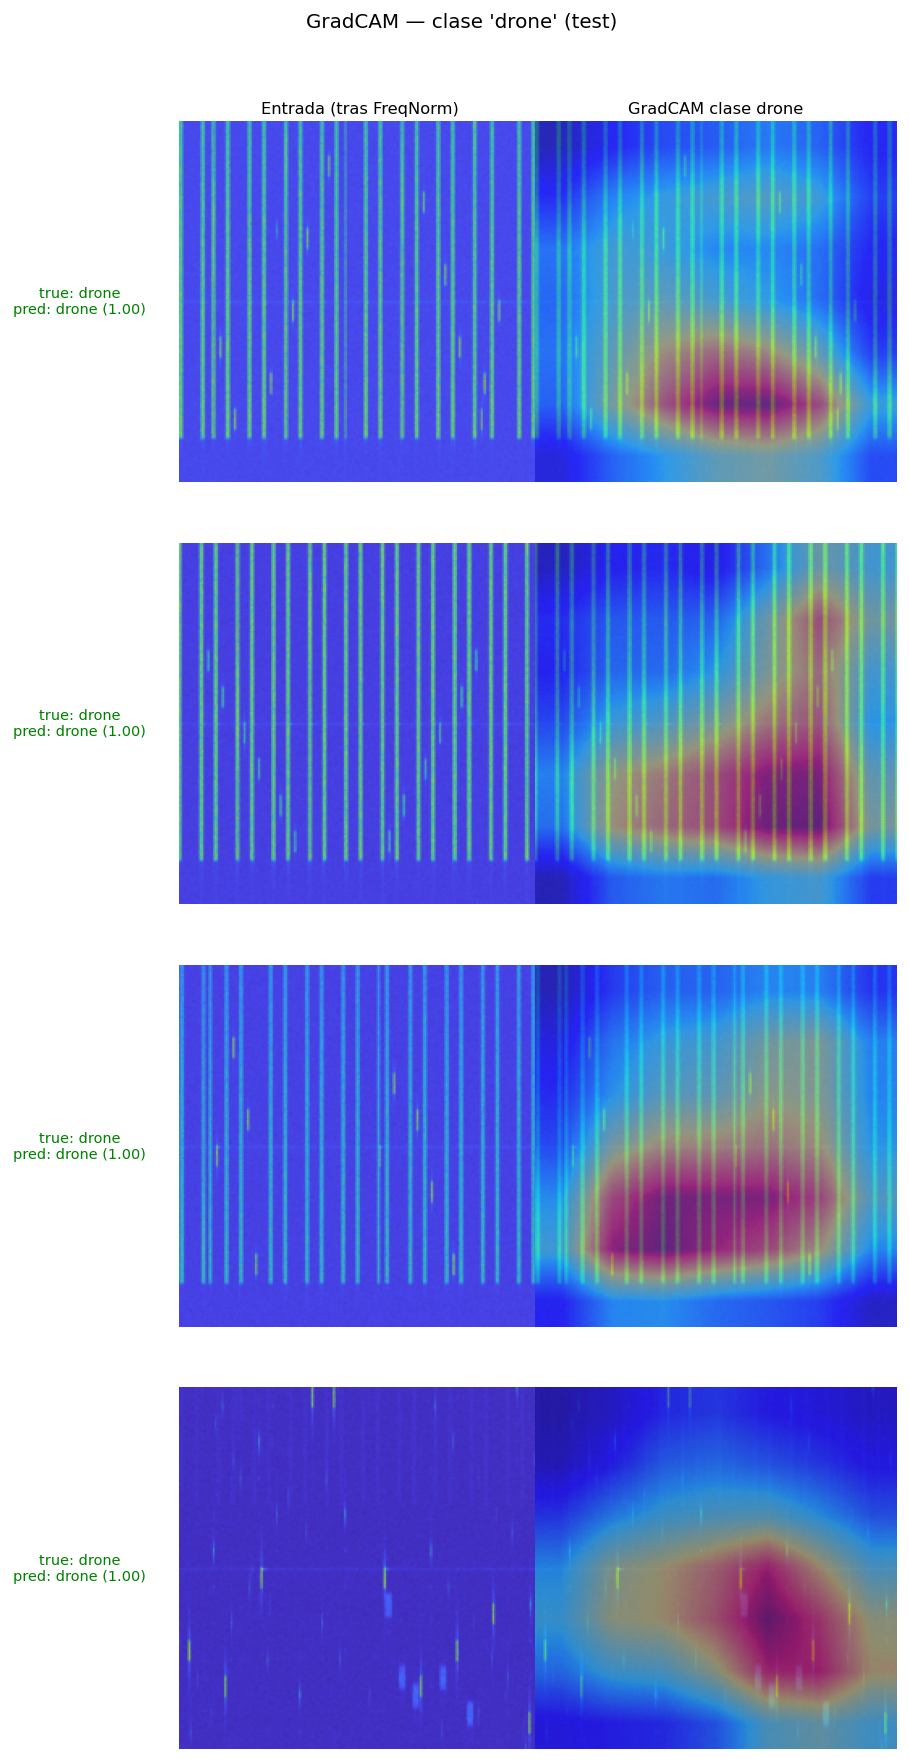
\includegraphics[width=0.80\textwidth]{figuras/resultados/gradcam_drone.png}
    \caption{GradCAM del clasificador ResNet18 binario sobre cuatro espectrogramas de la clase \emph{drone}. Izquierda: Ráfagas FHSS verticales de OcuSync claramente visibles. Derecha: mapa de calor de la clase \emph{drone}. }
    \label{fig:resnet18_gradcam_drone}
\end{figure}

\begin{figure}[htbp]
    \centering
    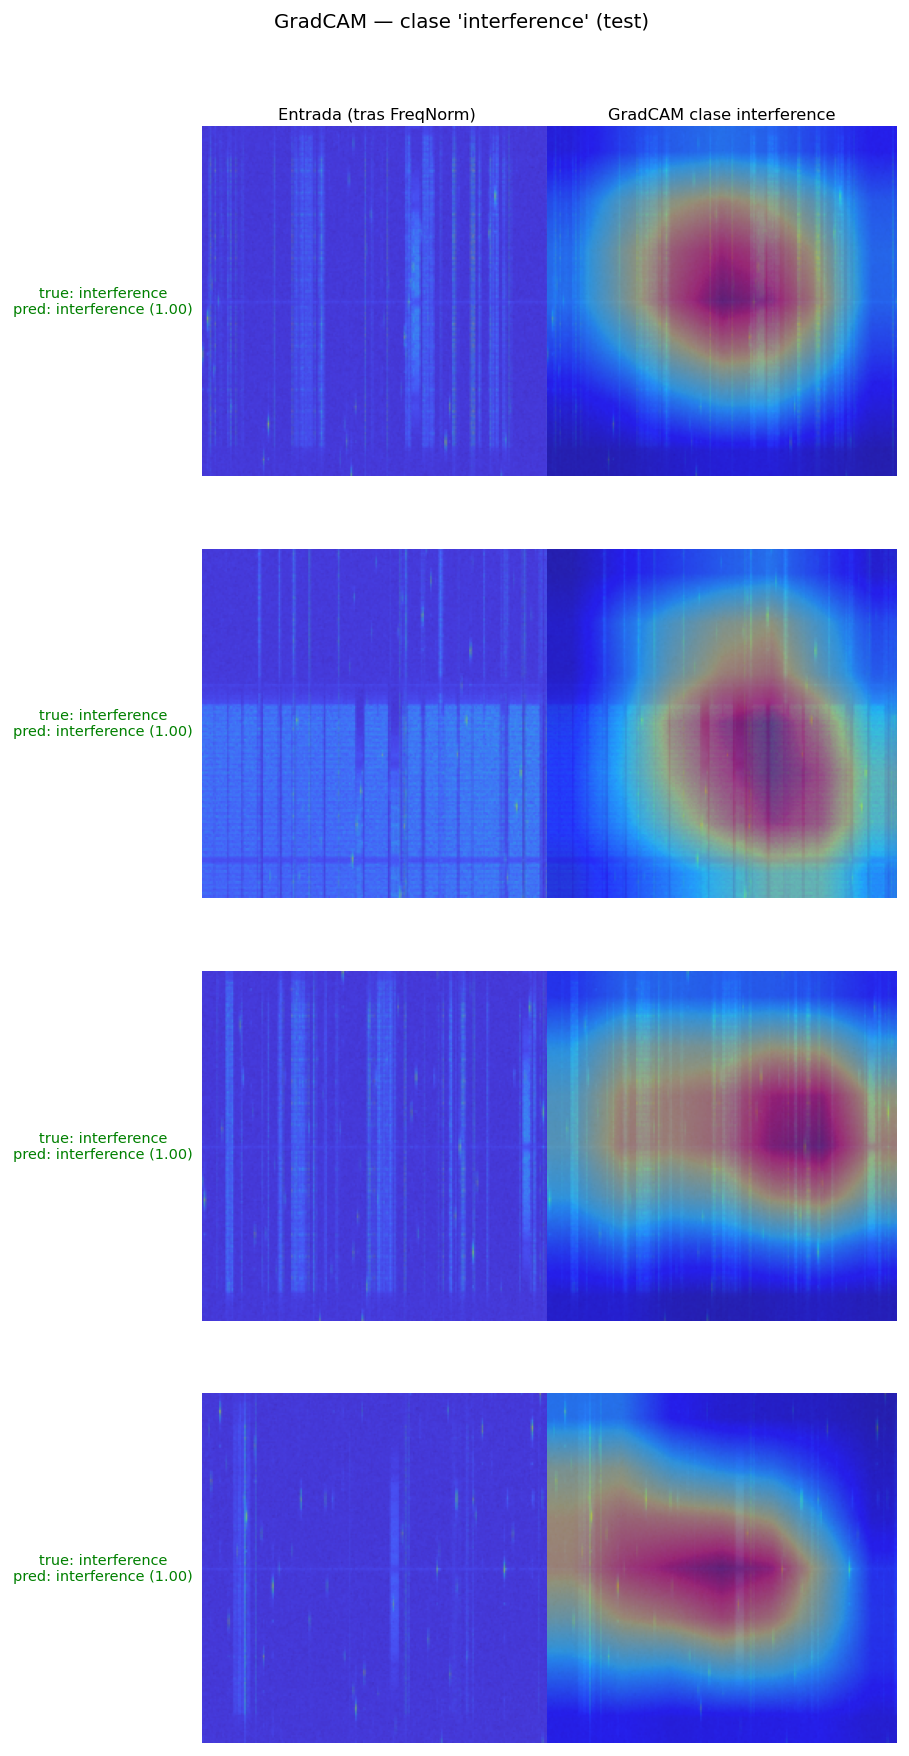
\includegraphics[width=0.80\textwidth]{figuras/resultados/gradcam_interference.png}
    \caption{GradCAM del clasificador ResNet18 binario sobre cuatro espectrogramas de la clase \emph{interference}. Izquierda: entrada tras \texttt{FrequencyNormalize}, con señales WiFi y Bluetooth dispersas y de menor energía. Derecha: mapa de calor de la clase \emph{interference}.}
    \label{fig:resnet18_gradcam_interference}
\end{figure}

El resultado es revelador y contrario a lo que cabría esperar de un modelo que hubiese aprendido la firma RF. En las capturas de dron (\cref{fig:resnet18_gradcam_drone}) la activación no recae sobre las ráfagas FHSS: forma una mancha difusa y suave en la región central-inferior que ignora la estructura vertical periódica de OcuSync y deja fuera las ráfagas de los bordes. En las capturas de interferencia (\cref{fig:resnet18_gradcam_interference}) el mapa de calor es esencialmente el mismo --- una mancha central de forma y posición casi indistinguibles --- a pesar de que el contenido de las dos imágenes no tiene nada en común.

La conclusión es directa: \textbf{los dos mapas de calor son prácticamente iguales entre clases}. Si la red estuviera discriminando por la morfología de la señal, el GradCAM de cada clase debería localizarse sobre estructuras distintas; en cambio, ambas predicciones se sustentan sobre la misma región central genérica de la imagen. GradCAM no consigue señalar ninguna evidencia local, específica de clase, que justifique la decisión. El clasificador alcanza F1\,=\,\num{1,000}, pero su atención no está anclada a la firma OcuSync, sino a un atributo difuso y global del espectrograma.

\subsection{Discusión}
\label{sec:p1_discusion}

El experimento P1 deja dos conclusiones. Por un lado, confirma que las dos clases son perfectamente separables con la información del espectrograma completo: la exactitud del \SI{100}{\percent} demuestra que existe alguna característica que distingue sin error una captura con dron de una de interferencia. Por otro lado, el análisis GradCAM demuestra que \textbf{esa característica no es la morfología de las ráfagas FHSS}. Una exactitud perfecta acompañada de mapas de saliencia difusos e idénticos entre clases es la huella típica de un clasificador que ha aprendido un atributo global de la captura --- nivel medio de potencia, brillo de fondo, condiciones del entorno de grabación --- correlacionado con la etiqueta pero ajeno a la señal del dron.


Este hallazgo es precisamente lo que invalida la clasificación global como criterio de detección, por tres motivos que se refuerzan entre sí.

El primero es la falta de auditabilidad. Un sistema de vigilancia debe poder justificar cada alarma señalando la evidencia concreta que la motiva. Un clasificador cuyo GradCAM apunta a una mancha central inespecífica no ofrece ninguna justificación verificable: no se puede saber qué parte de la señal ha disparado la decisión, ni distinguir una detección legítima de una casualidad estadística del conjunto de datos.


El segundo es la fragilidad ante el cambio de dominio. Si la decisión se apoya en un atributo global del entorno de captura y no en la firma RF, basta con que cambien las condiciones de grabación --- otra ganancia, otro recinto, exterior en lugar de interior --- para que la correlación aprendida se rompa y el rendimiento se desplome, aun cuando la señal del dron sea idéntica. La poca variabilidad intraclase del dataset~v3 (un único modelo de dron, un único entorno interior) hace que el atajo sea especialmente fácil de aprender y, por tanto, especialmente engañoso: el F1\,=\,\num{1,000} mide la capacidad de separar \emph{estas} capturas, no la de reconocer la firma de un dron en general.


El tercero es la ausencia de localización y de aprendizaje multietiqueta. El clasificador emite una única etiqueta para toda la imagen, de modo que no puede indicar en qué región del espectrograma está la señal ni representar la coexistencia de dron e interferencia en la misma ventana temporal, una situación habitual en un escenario real.


En conjunto, P1 demuestra que la pregunta «¿es la firma OcuSync separable?» tiene respuesta afirmativa, pero que un clasificador global no es la herramienta adecuada para responderla de forma fiable: acierta por las razones equivocadas. Estas limitaciones motivan directamente el experimento P2 --- reformular la tarea como detección de objetos ---, que obliga al modelo a justificar cada predicción con la región concreta del espectrograma que la soporta y, con ello, a aprender la morfología local de las ráfagas en lugar de un atajo contextual.








%=========================================================
\section{P2 --- ¿Puede YOLOv8 localizar y separar morfológicamente las ráfagas FHSS?}
\label{sec:bloque_yolo}

\subsection{Planteamiento del experimento}
\label{sec:p2_planteamiento}

El segundo experimento reformula el reconocimiento de señales como un problema de detección de objetos. En lugar de asignar una etiqueta global a cada espectrograma, el modelo debe generar cajas delimitadoras sobre las ráfagas individuales del plano tiempo-frecuencia y clasificar cada una como \emph{drone} (ráfaga OcuSync) o \emph{interference} (ráfaga WiFi/Bluetooth). Las etiquetas se generan con el auto-etiquetado descrito en la \cref{sec:autoetiquetado} (umbral percentil 99,8, etiquetado débil por captura), y el detector se configura según la \cref{sec:entrenamiento_yolo} (YOLOv8n, entrada 640×640, lote~16, sin aumentaciones geométricas).

Se realizan dos entrenamientos sobre el mismo dataset: una primera tanda de \num{15}~épocas como referencia inicial, y una segunda tanda de \num{60}~épocas como modelo final.

Las métricas de precisión, recall y mAP se definen en la \cref{subsec:diseno_evaluacion}. Conviene precisar aquí la distinción entre métricas globales y por clase: el \textbf{mAP@50 global} promedia la precisión media de cada clase activa sobre el conjunto de prueba; el \textbf{mAP@50 por clase} permite comparar directamente el rendimiento del detector sobre \emph{drone} frente a \emph{interference}. La \textbf{puntuación de confianza} (\emph{confidence score}) es el valor entre 0 y 1 que el modelo asigna a cada detección; se emplea como umbral de filtrado para controlar el equilibrio entre precisión y recall, y su elección óptima se determina a partir de la curva F1-confianza mostrada en los resultados.

\subsection{Resultados}
\label{sec:p2_resultados}

\paragraph{Evolución del entrenamiento.}

La \cref{fig:yolo_run02_results} muestra las curvas de pérdida y métricas de validación a lo largo de las \num{60}~épocas del modelo final.

\begin{figure}[htbp]
    \centering
    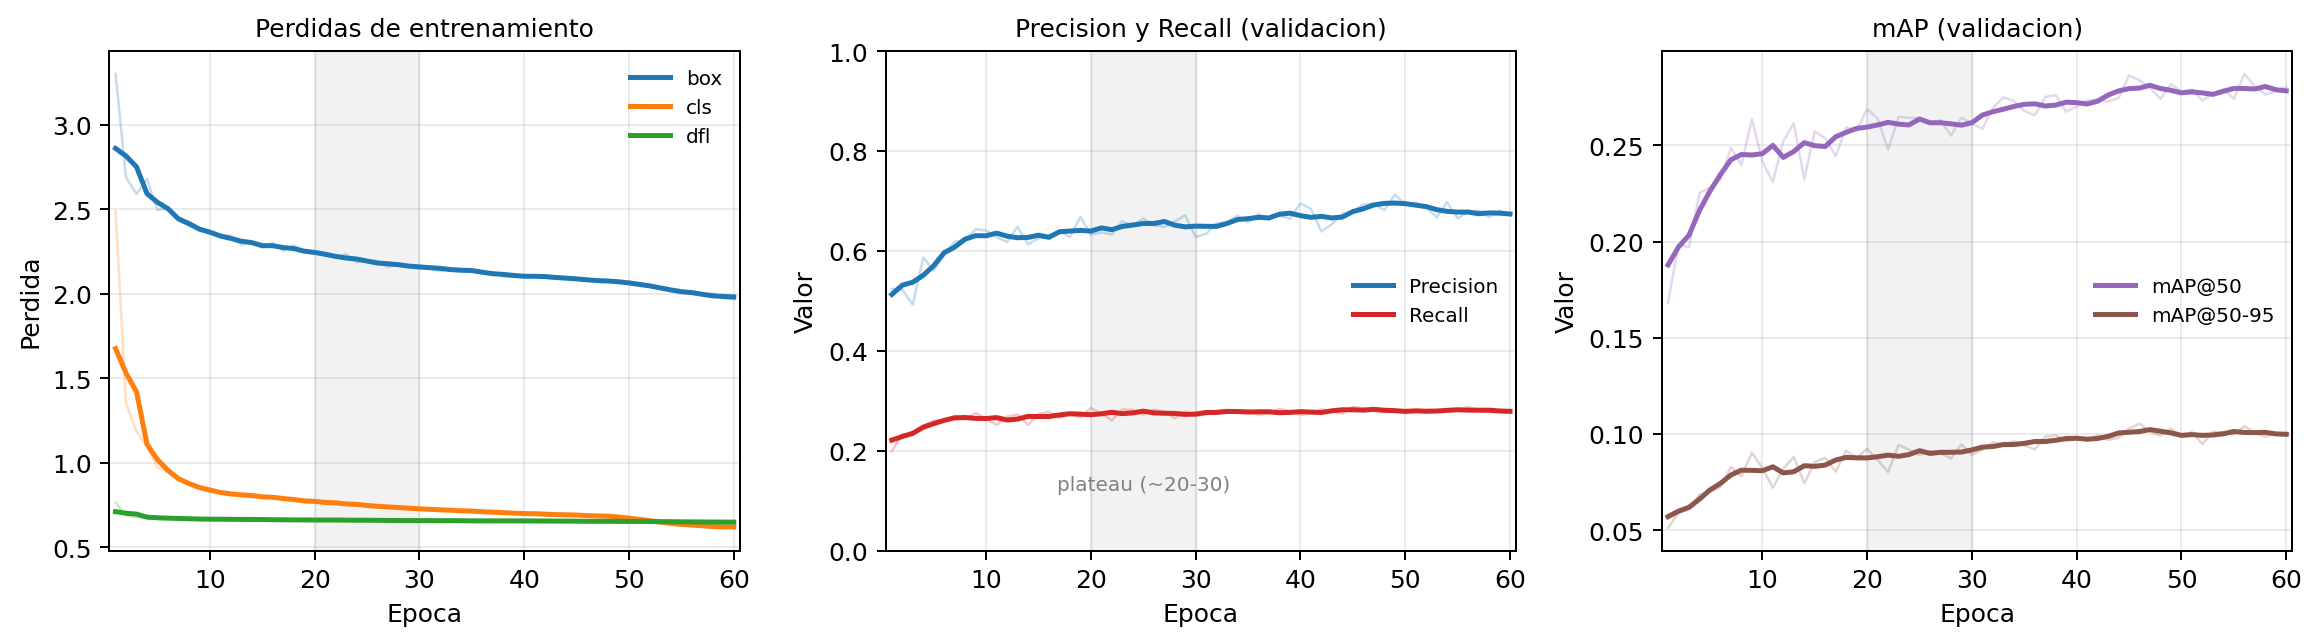
\includegraphics[width=\textwidth]{figuras/resultados/yolo_run02_curvas.png}
    \caption{Evolución del entrenamiento del detector YOLOv8n a lo largo de las \num{60}~épocas (tanda~2), resumida en tres paneles. Izquierda: las tres pérdidas de entrenamiento (box, cls, dfl) descienden de forma continua. Centro: la precisión y el recall de validación se estabilizan en una meseta aproximadamente entre las épocas 20 y 30 (banda sombreada). Derecha: el mAP@50 y el mAP@50-95 de validación siguen el mismo patrón; las épocas adicionales aportan una leve mejora de la precisión geométrica de las cajas (mAP@50-95) sin aumentar de forma significativa la cobertura (recall, mAP@50). En cada panel la línea tenue son los valores por época y la gruesa la tendencia suavizada.}
    \label{fig:yolo_run02_results}
\end{figure}

Las curvas muestran un comportamiento saludable: las pérdidas de entrenamiento descienden de forma continua y no hay señales de sobreajuste severo. Las métricas de validación se estabilizan entre las épocas~20 y~30 sin tendencia creciente clara a partir de ese punto. Esto indica que el límite del experimento no reside en la duración del entrenamiento, sino en la dificultad intrínseca del problema --- tamaño de las ráfagas en el espectrograma y ruido en el etiquetado automático ---, que las épocas adicionales no pueden superar.

\paragraph{Comparativa entre tandas.}

La \cref{tab:comparativa_epochs} compara los resultados de test de ambas tandas de entrenamiento.

\begin{table}[htbp]
\centering
\caption{Comparativa de resultados sobre el conjunto de prueba entre la tanda de \num{15}~épocas y la de \num{60}~épocas.}
\label{tab:comparativa_epochs}
\begin{tabular}{lccc}
\toprule
\textbf{Métrica} & \textbf{15 épocas} & \textbf{60 épocas} & \textbf{Diferencia} \\
\midrule
Precisión global        & 0,748 & 0,760 & +0,012 \\
Recall global           & 0,395 & 0,391 & $-$0,004 \\
mAP@50 global           & 0,386 & 0,388 & +0,002 \\
mAP@50-95 global        & 0,195 & 0,203 & +0,008 \\
mAP@50 drone            & 0,571 & 0,575 & +0,004 \\
mAP@50-95 drone         & 0,333 & 0,348 & +0,015 \\
mAP@50 interference     & 0,201 & 0,201 & $\pm$0,000 \\
mAP@50-95 interference  & 0,056 & 0,058 & +0,002 \\
\bottomrule
\end{tabular}
\end{table}

La tanda de \num{60}~épocas aporta una mejora marginal en la mayoría de métricas, siendo más apreciable en mAP@50-95 para \emph{drone} (+0,015). Esto es coherente con las curvas de la \cref{fig:yolo_run02_results}: las épocas adicionales refinan la localización geométrica de las cajas de dron sin aumentar el número de ráfagas detectadas.

\FloatBarrier
\paragraph{Separabilidad entre clases: matriz de confusión.}

La matriz de confusión normalizada constituye el resultado más relevante del experimento para responder a P2. En la matriz, las filas corresponden a las clases reales y las columnas a las clases predichas (incluyendo \emph{background}). Los valores de la diagonal indican la tasa de acierto de cada clase; los valores fuera de la diagonal entre dos clases activas indican confusión cruzada entre ellas; los valores en la columna \emph{background} indican ráfagas reales no detectadas.

\begin{figure}[htbp]
    \centering
    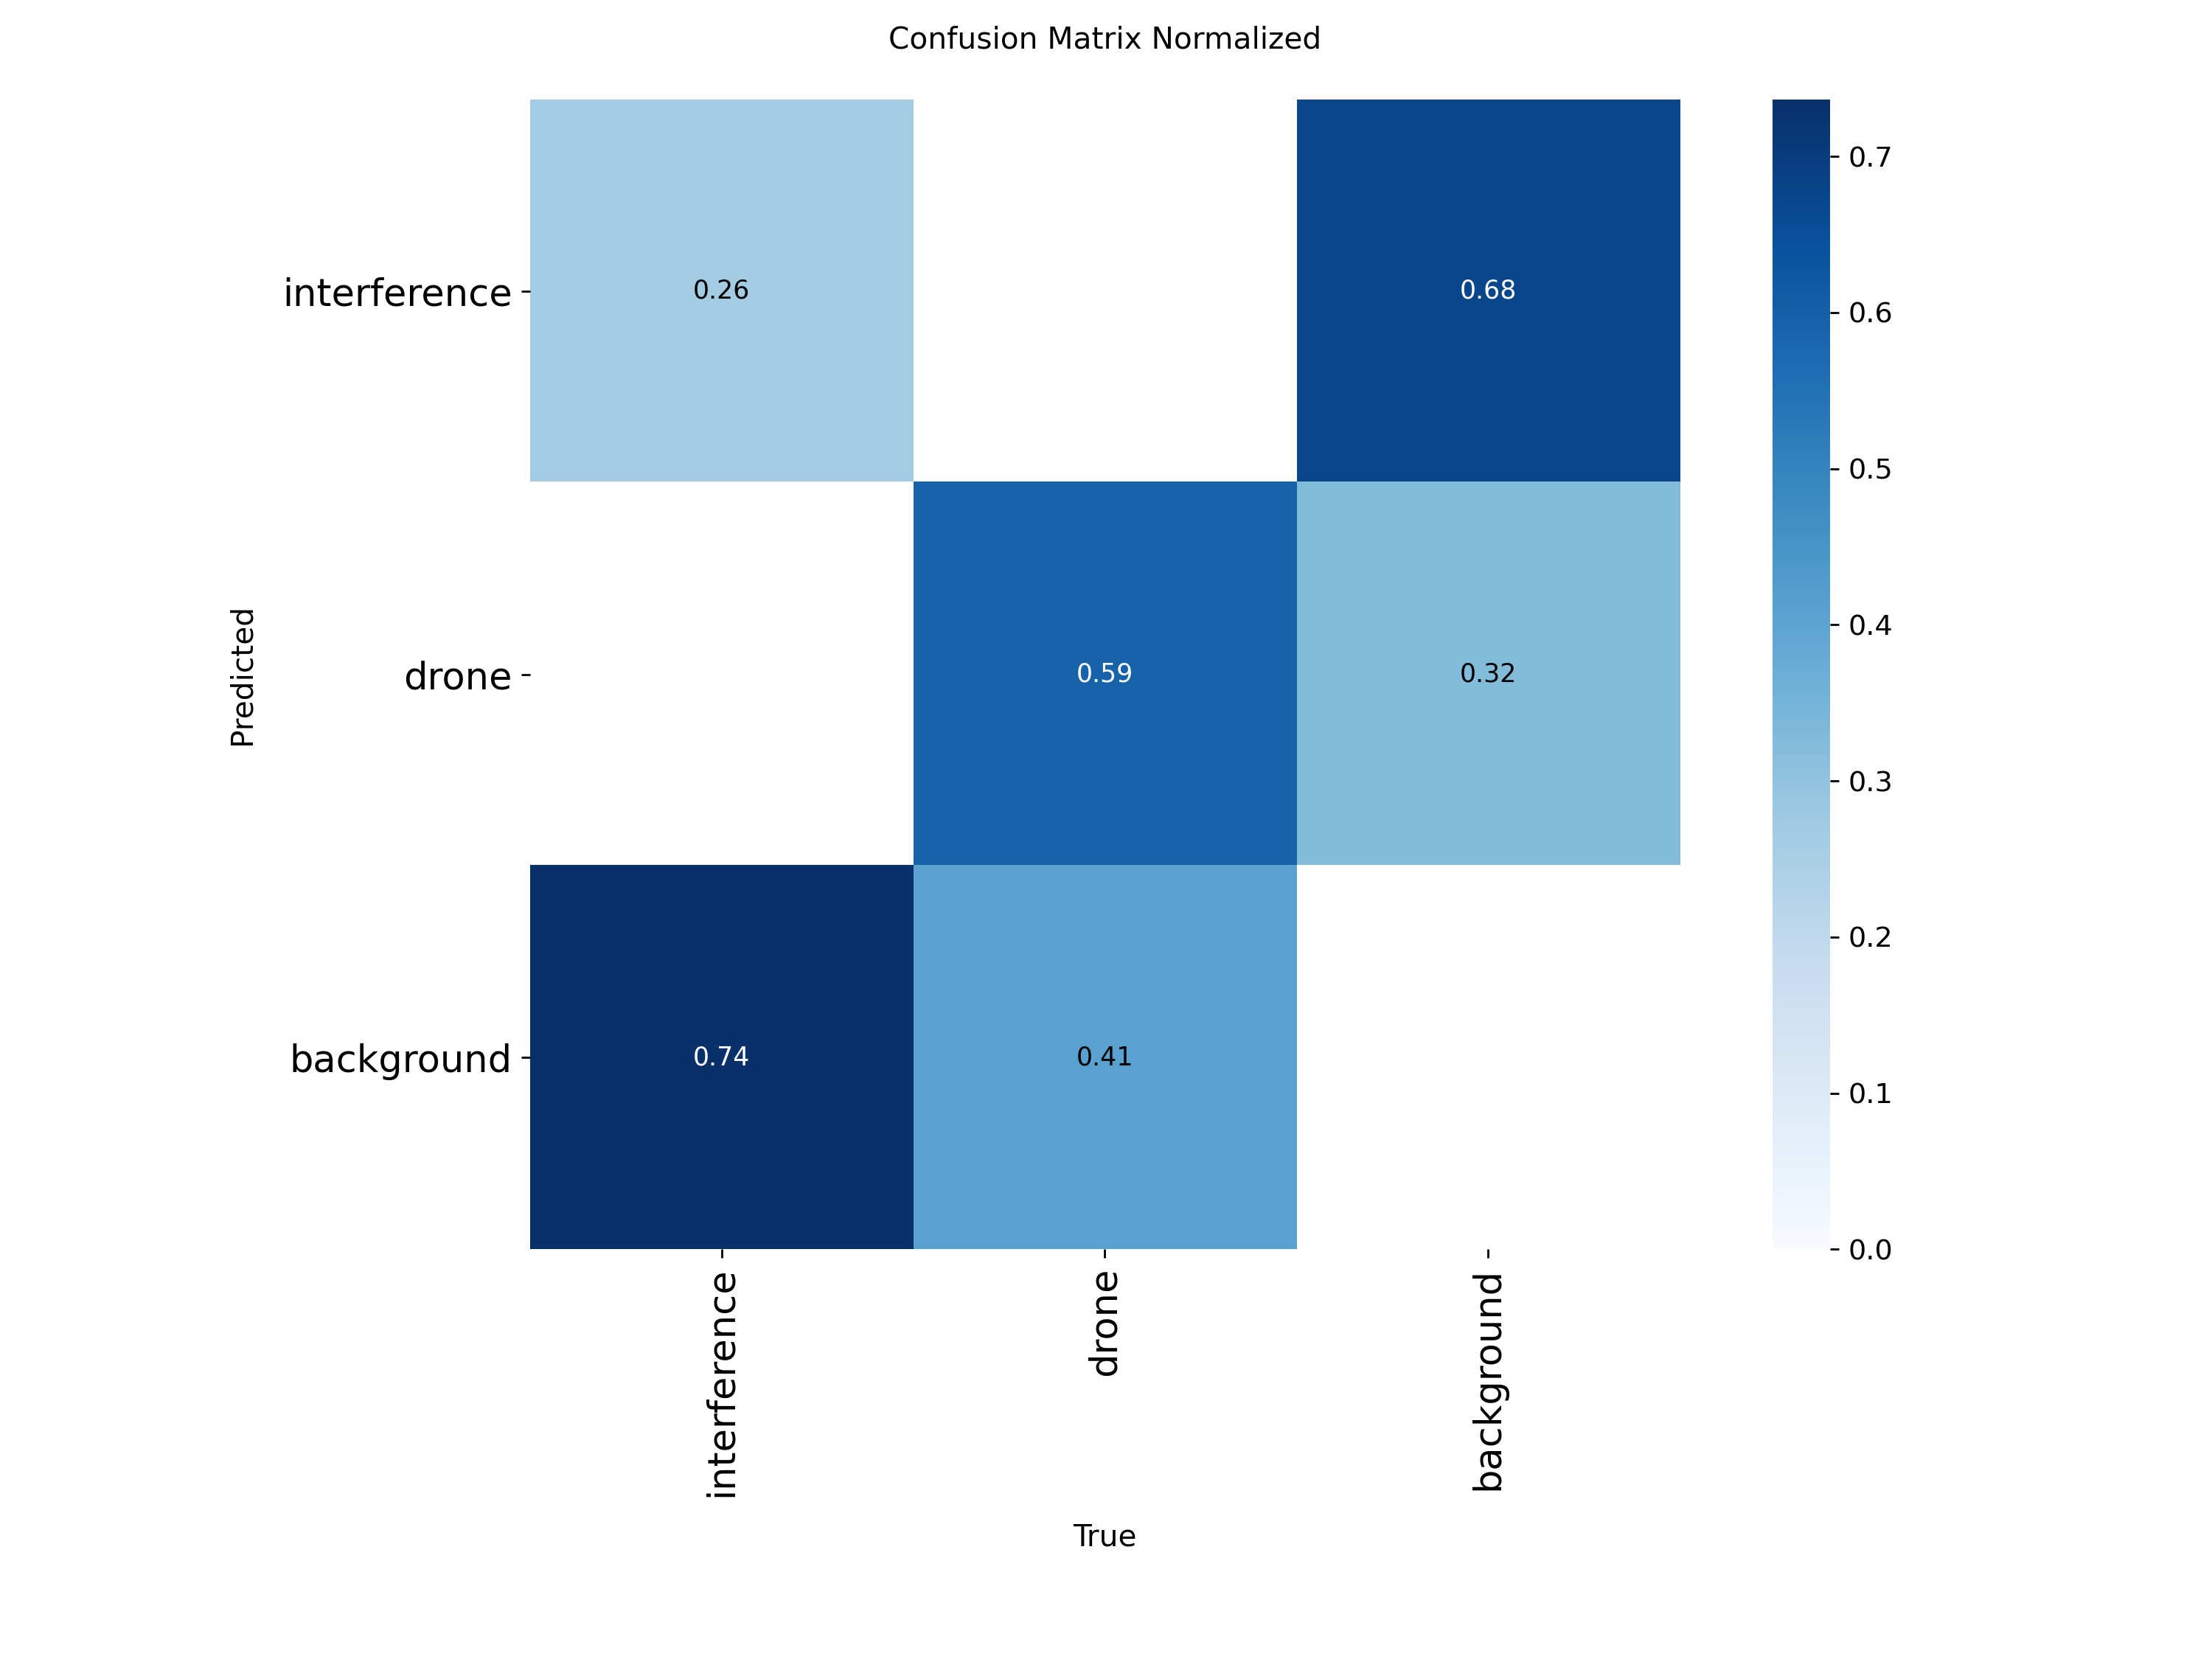
\includegraphics[width=0.75\textwidth]{figuras/resultados/confusion_matrix_normalized.png}
    \caption{Matriz de confusión normalizada del detector YOLOv8n sobre el conjunto de prueba. No se observa confusión cruzada entre \emph{drone} e \emph{interference}: cuando el modelo emite una predicción positiva, la clase asignada es correcta. Los errores son íntegramente falsos negativos (ráfagas reales asignadas a \emph{background}).}
    \label{fig:confusion_matrix_normalized}
\end{figure}

La \cref{fig:confusion_matrix_normalized} revela el resultado central del experimento: no existe confusión cruzada entre \emph{drone} e \emph{interference}. Ninguna ráfaga real de OcuSync es clasificada como interferencia, y ninguna ráfaga de interferencia es clasificada como señal de dron. Las tasas de confusión cruzada son ambas 0,00. Los errores son íntegramente falsos negativos: la tasa de detección a nivel de caja es de 0,42 para \emph{drone} y de 0,18 para \emph{interference}, con el complemento asignado a \emph{background}.

\FloatBarrier
\paragraph{Curvas precisión-recall y F1-confianza.}

La \cref{fig:box_pr_curve} muestra la curva precisión-recall del detector para ambas clases. La curva resume el equilibrio entre precisión y recall al variar el umbral de confianza: a umbrales altos el modelo es más selectivo (mayor precisión, menor recall); a umbrales bajos acepta más detecciones (mayor recall, menor precisión).

\begin{figure}[htbp]
    \centering
    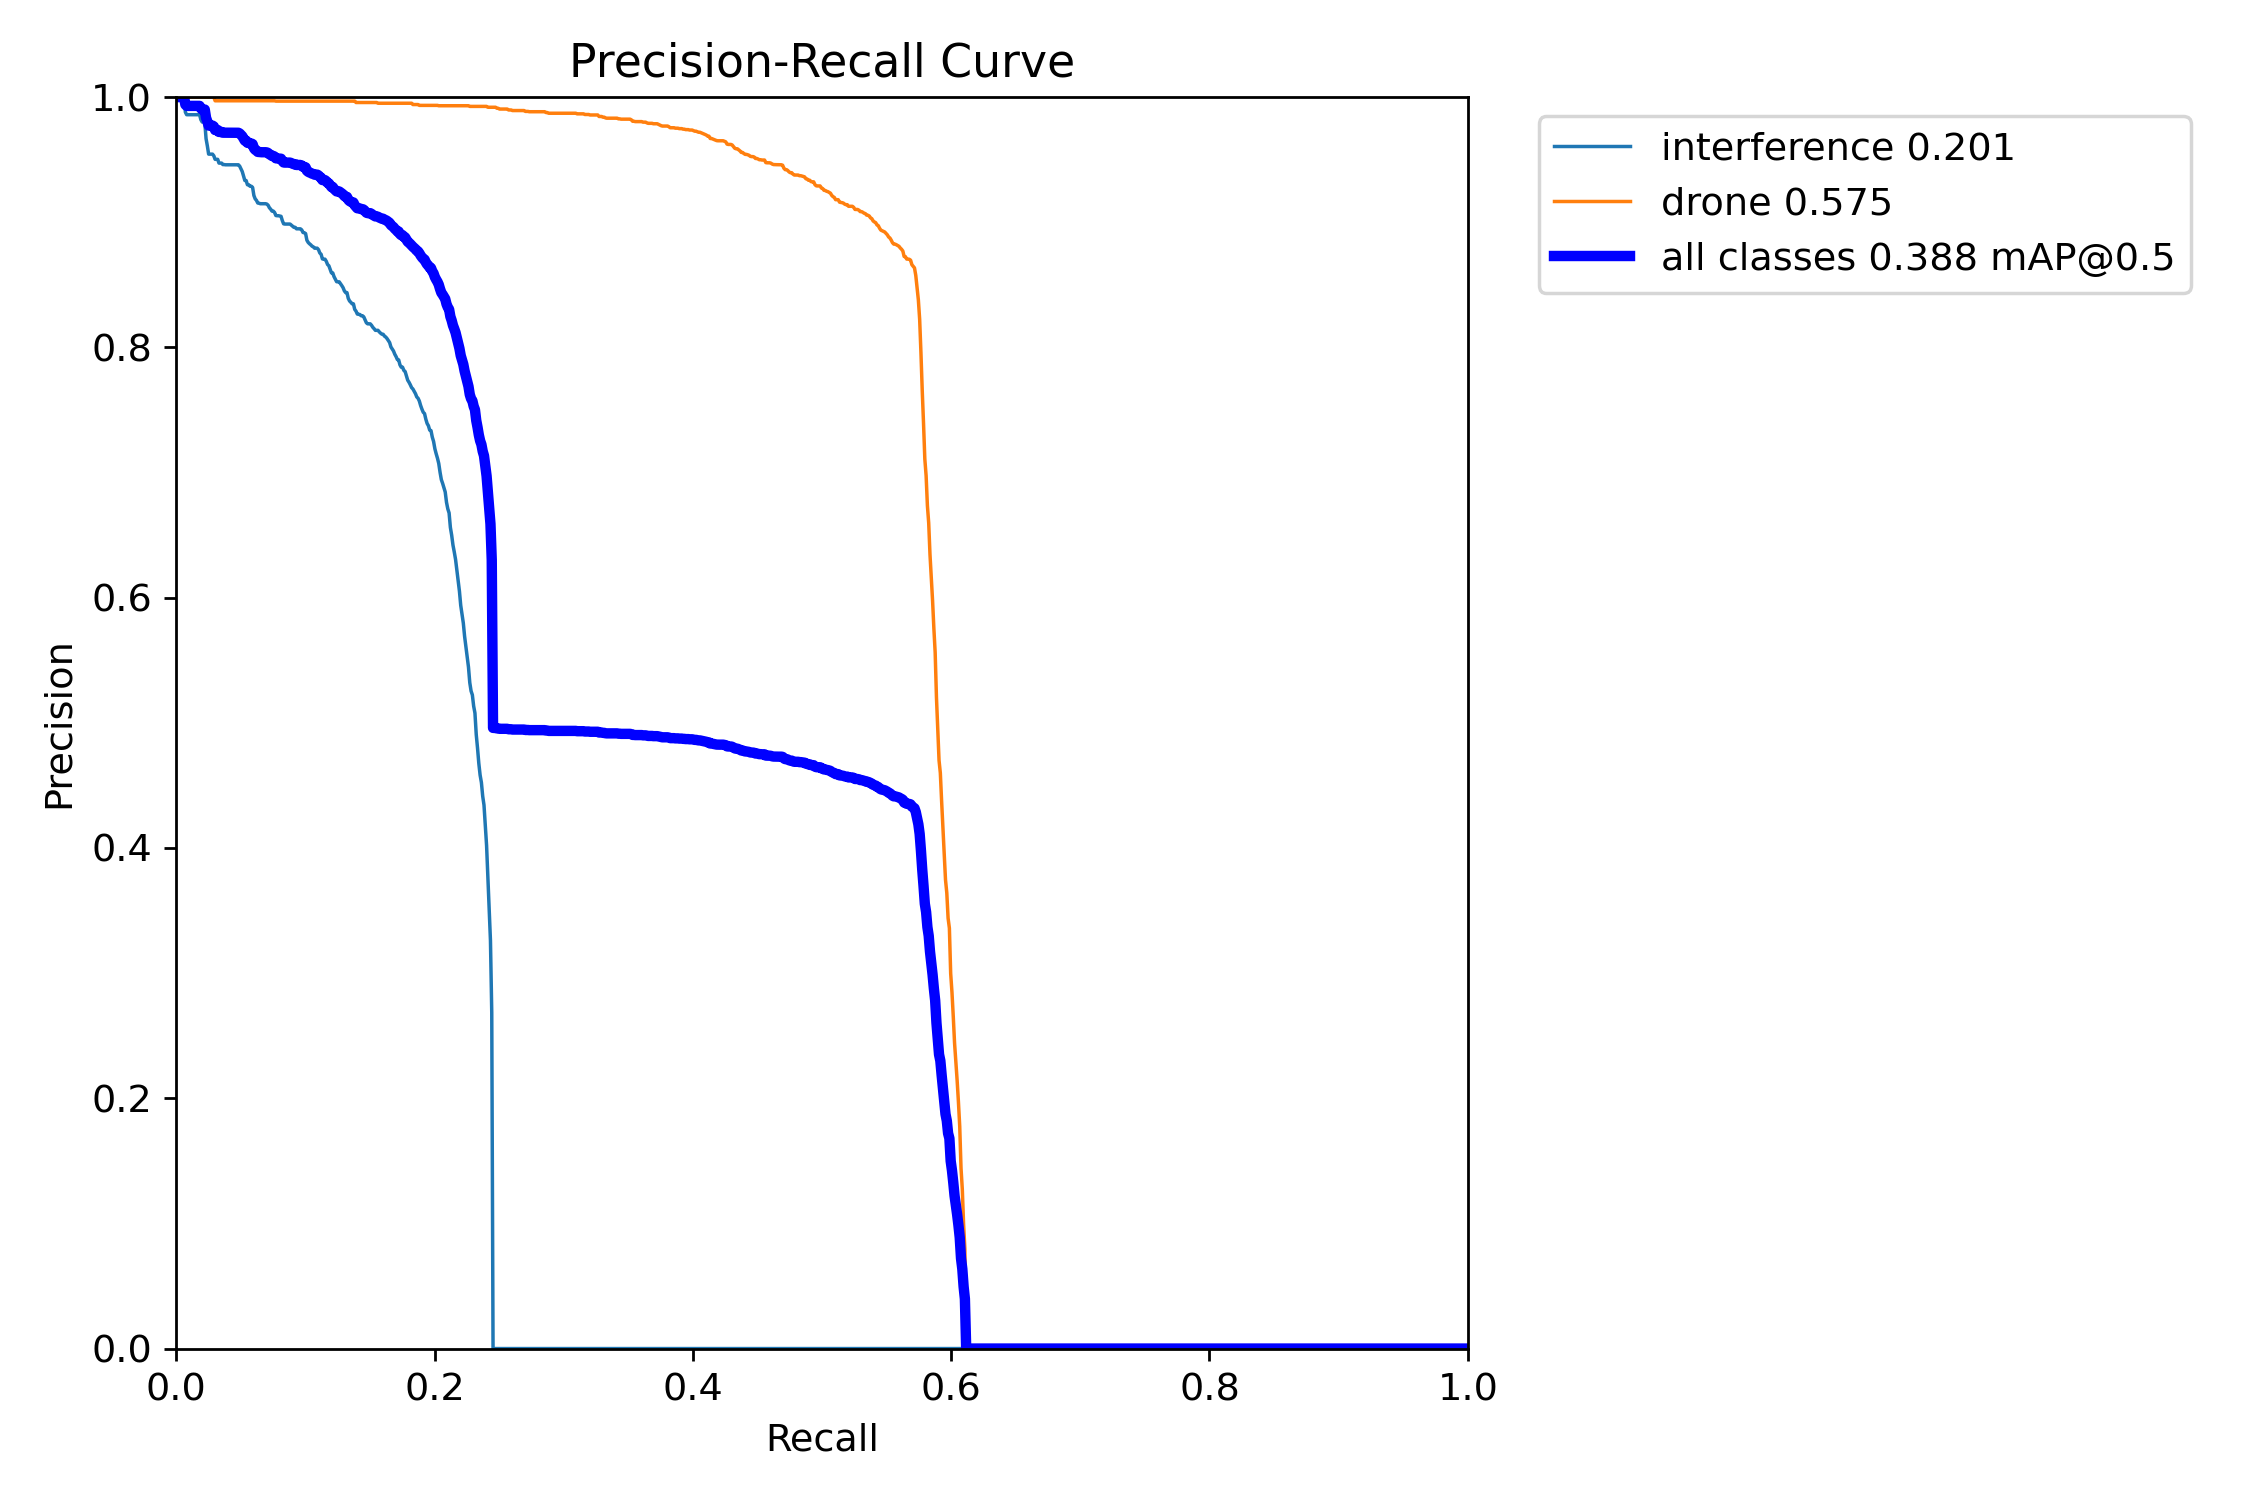
\includegraphics[width=0.85\textwidth]{figuras/resultados/BoxPR_curve.png}
    \caption{Curva precisión-recall del detector YOLOv8n sobre el conjunto de prueba. Cada punto corresponde a un umbral de confianza distinto. La clase \emph{drone} mantiene una precisión elevada en un rango de recall más amplio que \emph{interference}, lo que refleja la mayor homogeneidad de las ráfagas OcuSync respecto a las interferencias heterogéneas.}
    \label{fig:box_pr_curve}
\end{figure}

La \cref{fig:box_f1_curve} complementa la anterior mostrando el F1 en función del umbral de confianza. Esta curva permite identificar directamente el umbral que maximiza el F1 para cada clase o para el sistema global, y es la herramienta principal para seleccionar el punto de operación del sistema de detección. El máximo global se alcanza con umbrales de confianza bajos (en torno a 0,10-0,20), lo que indica que el detector asigna puntuaciones moderadas a una fracción relevante de ráfagas reales. En el experimento P3 se explotan explícitamente distintos valores de este umbral para determinar el punto de operación del clasificador de presencia.

\begin{figure}[htbp]
    \centering
    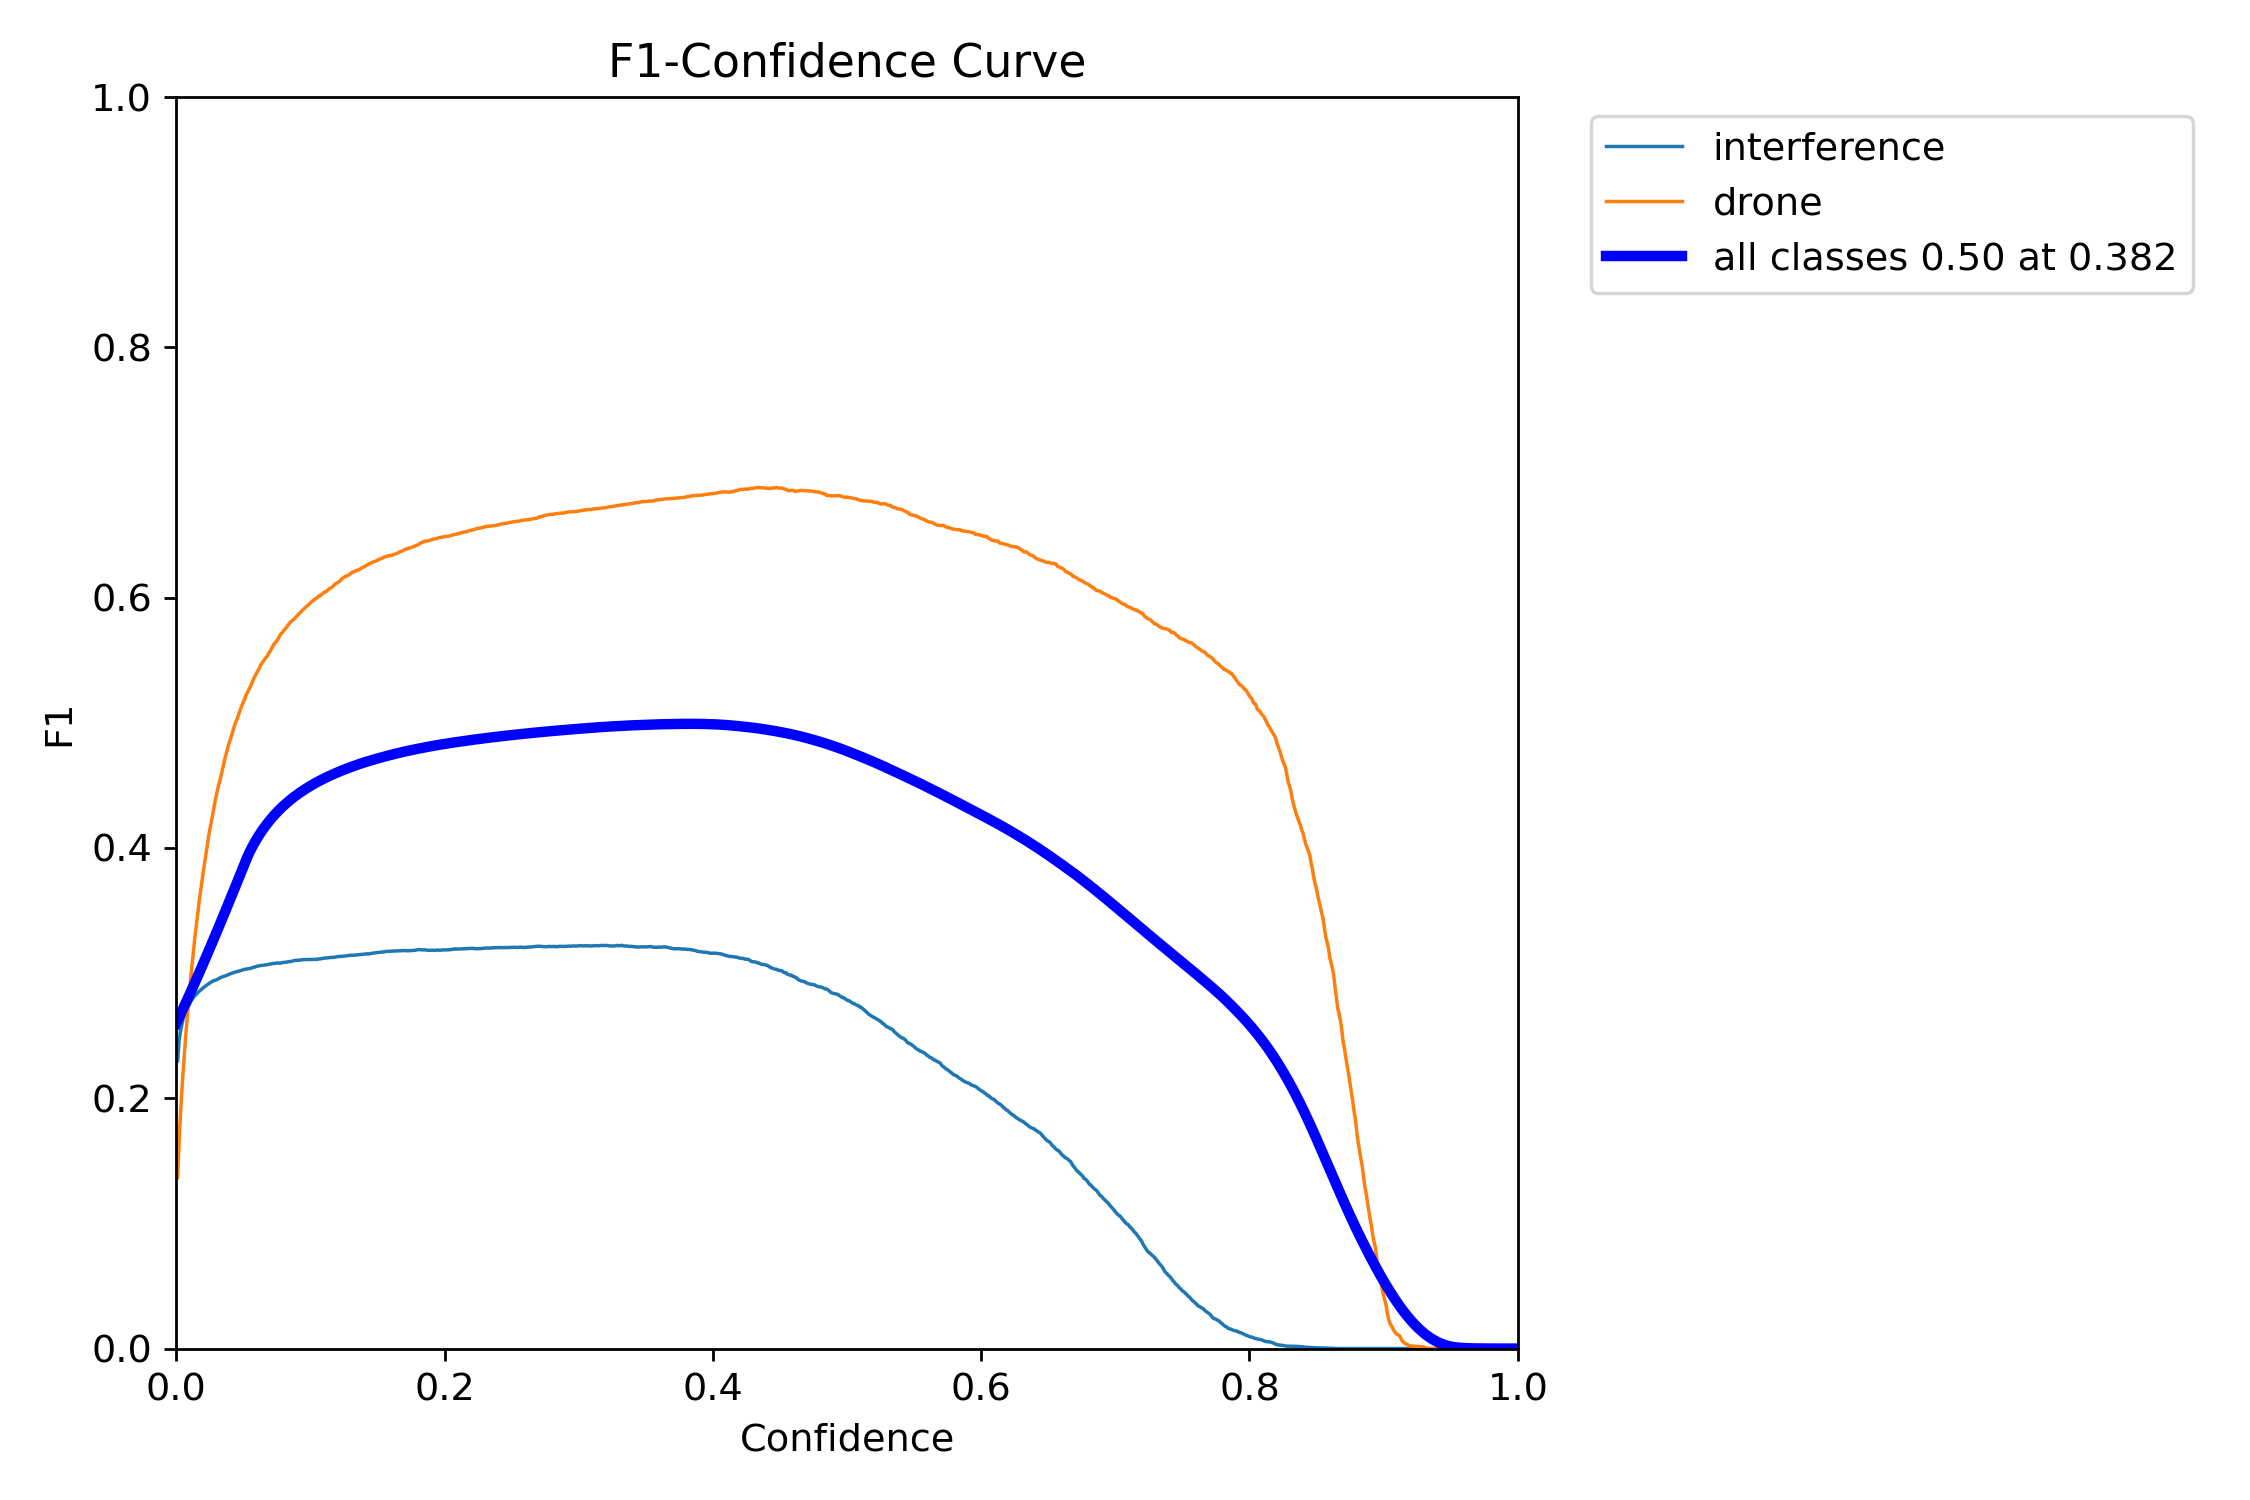
\includegraphics[width=0.85\textwidth]{figuras/resultados/BoxF1_curve.png}
    \caption{Curva F1-confianza del detector YOLOv8n. El eje horizontal representa el umbral de confianza mínimo para retener una detección, y el eje vertical el F1 resultante. El máximo global se alcanza con un umbral bajo, lo que indica que bajar el umbral recupera ráfagas reales sin penalizar excesivamente la precisión.}
    \label{fig:box_f1_curve}
\end{figure}

\FloatBarrier
\paragraph{Ejemplos cualitativos.}

Las \cref{fig:val_labels,fig:val_pred} comparan las etiquetas de referencia con las predicciones del modelo sobre un mismo lote de validación, permitiendo verificar visualmente la coherencia entre las métricas agregadas y el comportamiento sobre espectrogramas concretos.

\begin{figure}[htbp]
    \centering
    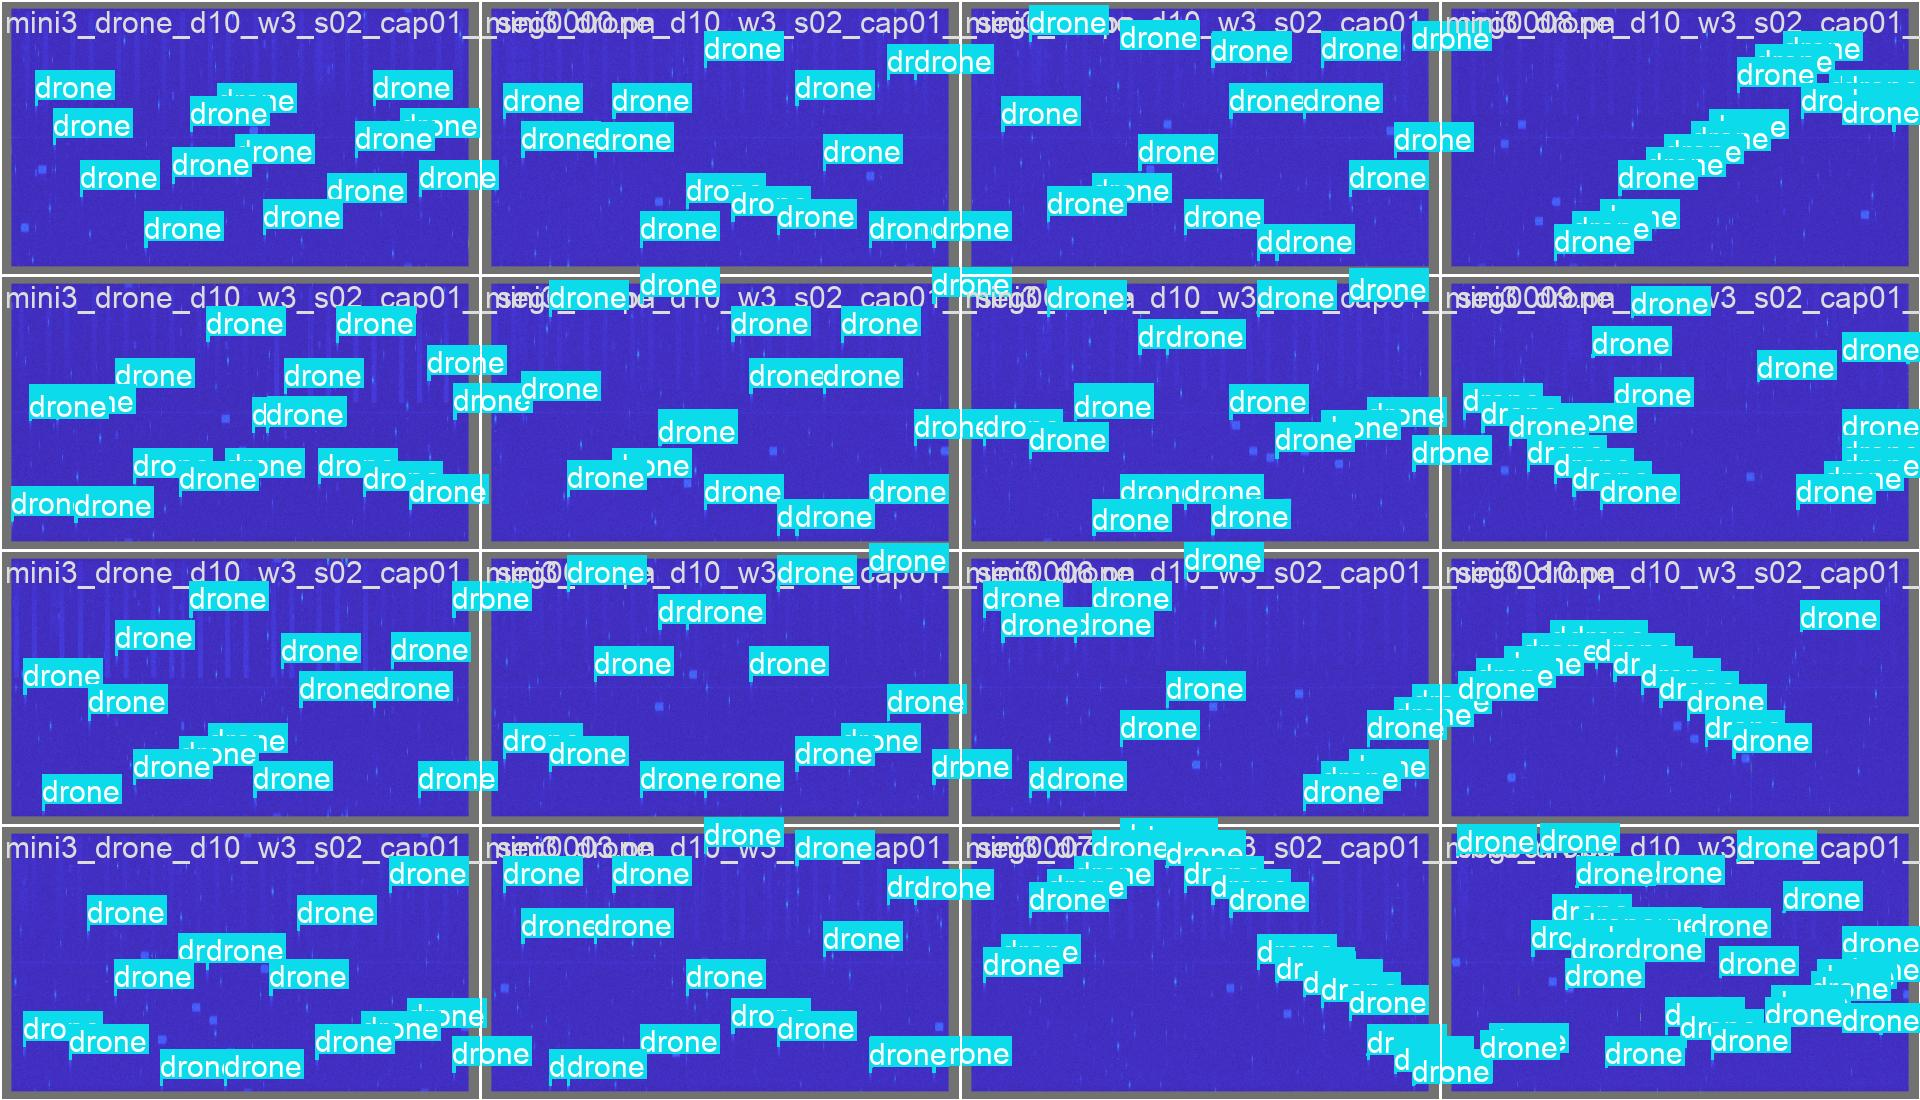
\includegraphics[width=0.9\textwidth]{figuras/resultados/val_batch0_labels.jpg}
    \caption{Etiquetas de referencia (\emph{ground truth}) sobre un lote de validación de capturas de dron. Cada caja delimita una ráfaga FHSS de OcuSync generada por el auto-etiquetado.}
    \label{fig:val_labels}
\end{figure}

\begin{figure}[htbp]
    \centering
    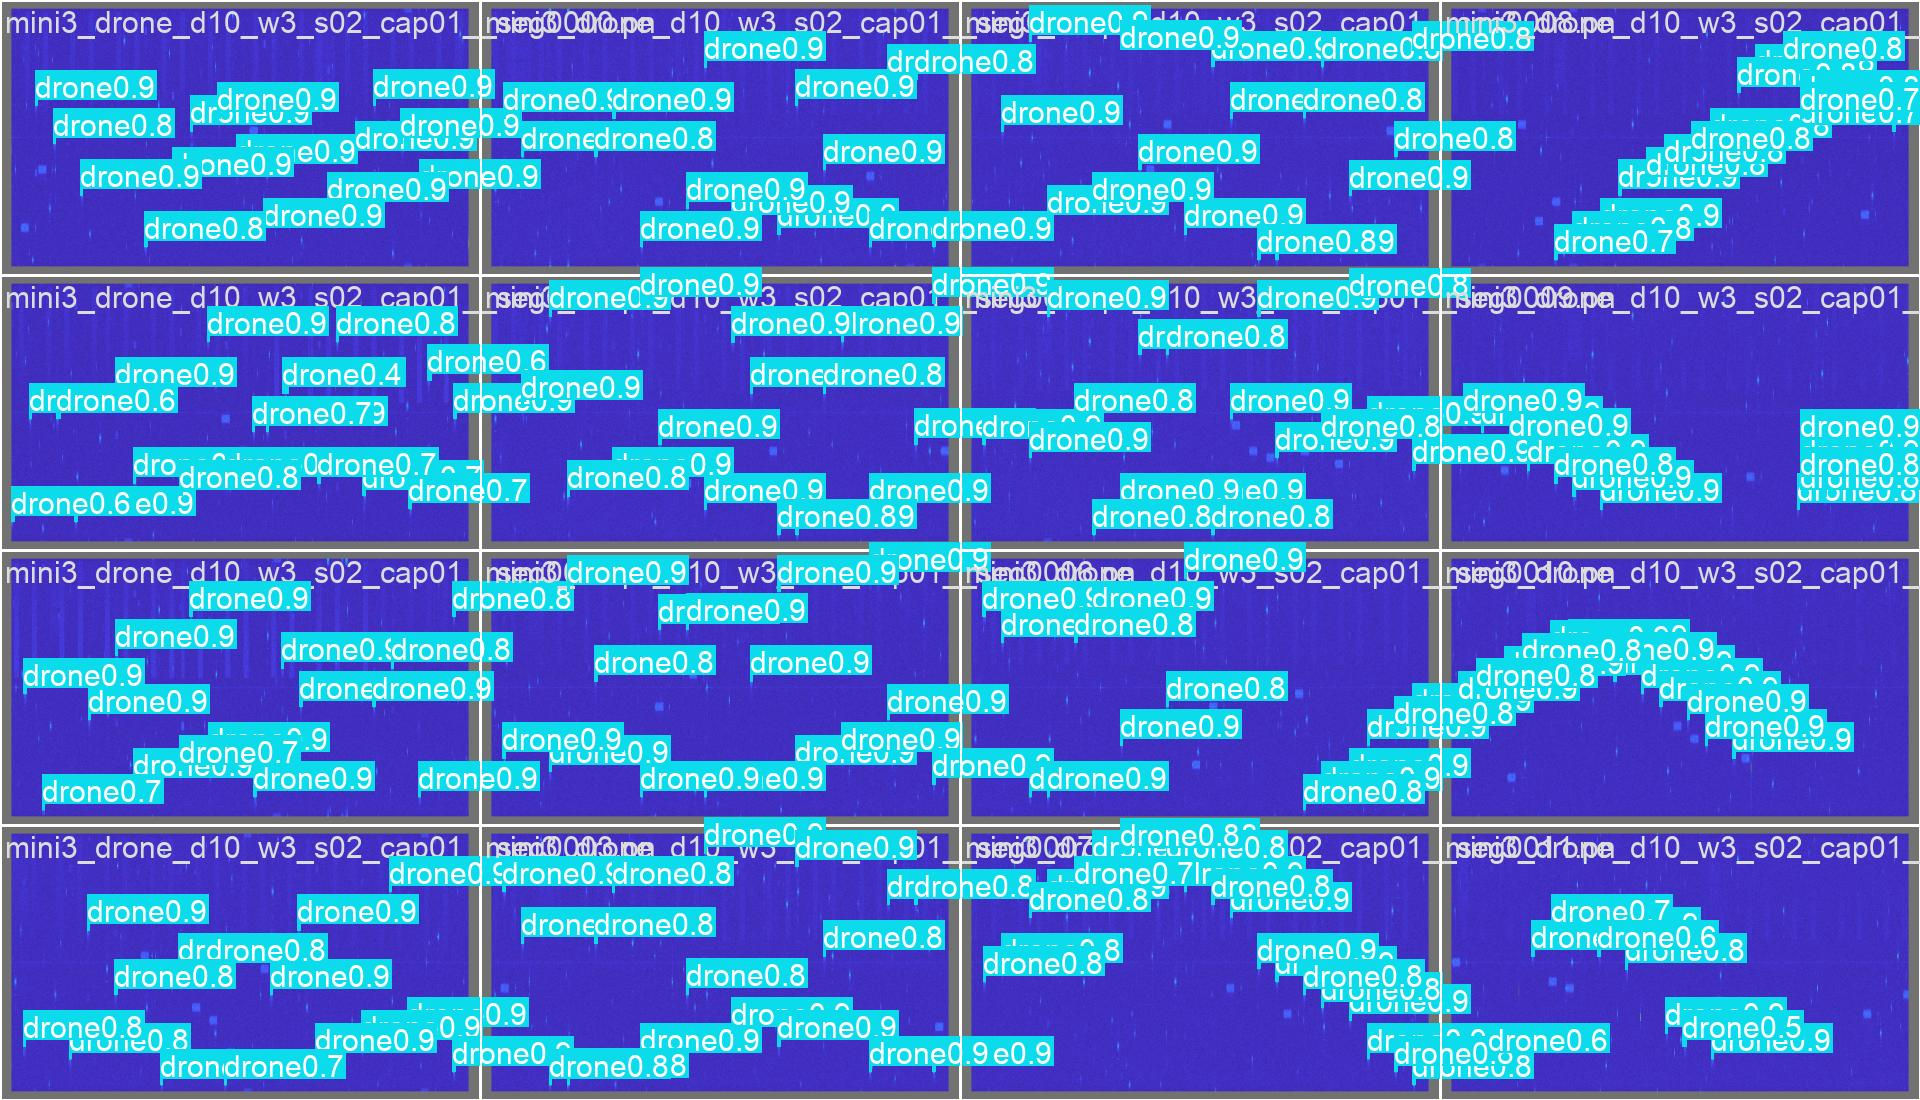
\includegraphics[width=0.9\textwidth]{figuras/resultados/val_batch0_pred.jpg}
    \caption{Predicciones del detector YOLOv8n sobre el mismo lote, con su puntuación de confianza asociada. Las cajas predichas se superponen sobre las mismas ráfagas FHSS que indican las etiquetas de referencia de la \cref{fig:val_labels}, con confianzas típicas entre 0,6 y 0,9. No aparecen cajas sobre regiones de fondo vacío: no hay falsos positivos.}
    \label{fig:val_pred}
\end{figure}

La comparación entre ambas figuras muestra que las cajas predichas se sitúan sobre las mismas ráfagas que las etiquetas de referencia. La densidad de cajas predichas es inferior a la de referencia, lo que es coherente con el recall de 0,39: el modelo no recupera todas las ráfagas etiquetadas. No aparecen, en cambio, cajas sobre regiones del espectrograma sin señal: no hay falsos positivos.

\FloatBarrier
\subsection{Interpretabilidad mediante EigenCAM}
\label{sec:eigencam}

Las métricas anteriores cuantifican el rendimiento del detector pero no revelan en qué características del espectrograma se apoya para inferir sus decisiones. Esta información es relevante para la auditabilidad del sistema: en aplicaciones de vigilancia, un detector debe poder justificar sus predicciones de forma verificable. Con este objetivo se aplica EigenCAM para analizar qué regiones del espectrograma activan internamente la red.

EigenCAM extrae las activaciones de la capa del cuello de YOLOv8 responsable de detectar objetos de tamaño pequeño y calcula su primera componente principal, produciendo un mapa de calor sobre el espectrograma. Al operar directamente sobre activaciones --- y no sobre gradientes respecto a ninguna clase objetivo ---, el mapa refleja las regiones que generan respuestas fuertes y coherentes en la red con independencia de la clase predicha.

\begin{figure}[htbp]
    \centering
    \begin{subfigure}[b]{0.48\textwidth}
        \centering
        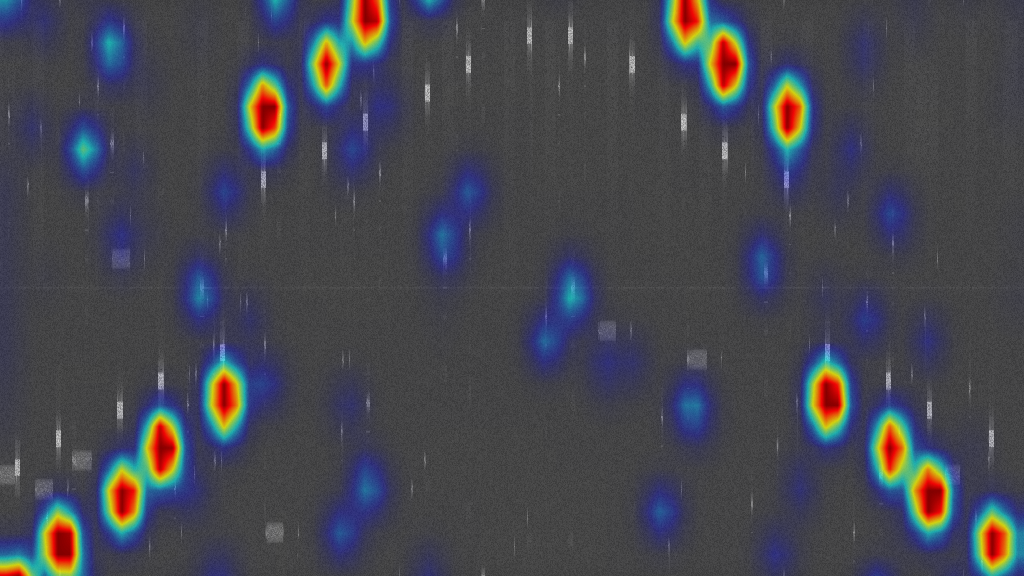
\includegraphics[width=\textwidth]{figuras/resultados/cam_drone_00.png}
        \caption{Captura con dron (protocolo OcuSync).}
        \label{fig:eigencam_drone}
    \end{subfigure}
    \hfill
    \begin{subfigure}[b]{0.48\textwidth}
        \centering
        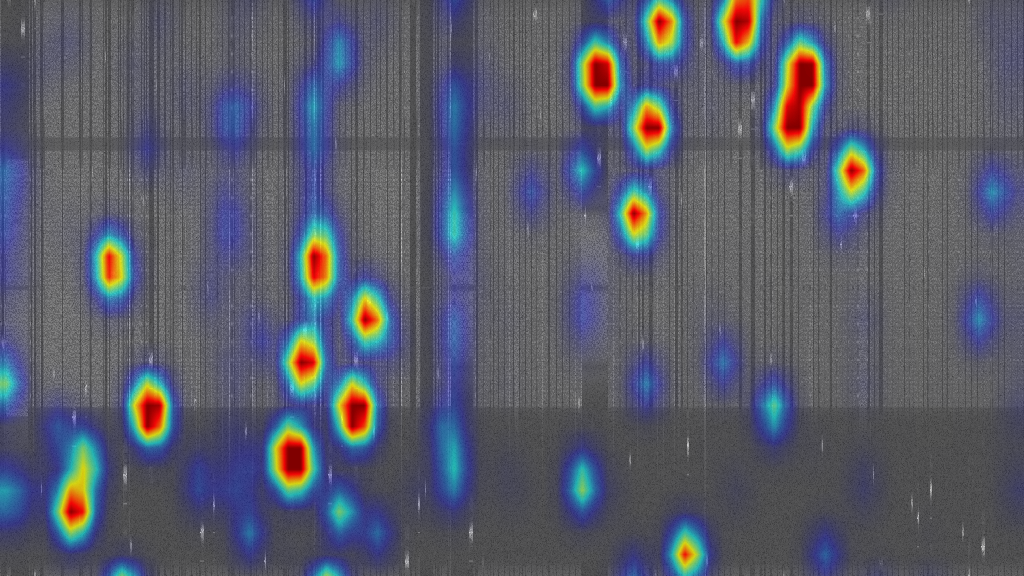
\includegraphics[width=\textwidth]{figuras/resultados/eigencam_interference.png}
        \caption{Captura de interferencia (WiFi/Bluetooth).}
        \label{fig:eigencam_interference}
    \end{subfigure}
    \caption{Mapas de saliencia EigenCAM del detector YOLOv8n sobre dos espectrogramas de prueba. El espectrograma subyacente se muestra en escala de grises y el color indica la intensidad de activación (rojo = alta, azul = baja). En la captura de dron, los focos de activación coinciden con las posiciones de las ráfagas OcuSync que las etiquetas de referencia de la \cref{fig:val_labels} delimitan como \emph{drone}. En la captura de interferencia, la activación recae sobre las estructuras WiFi y Bluetooth activas.}
    \label{fig:eigencam}
\end{figure}

La \cref{fig:eigencam} muestra los resultados para dos espectrogramas representativos del conjunto de prueba. En la captura de dron (\cref{fig:eigencam_drone}), los focos de calor son estructuras compactas que coinciden espacialmente con las ráfagas FHSS de OcuSync: las mismas posiciones que las etiquetas de referencia de la \cref{fig:val_labels} identifican como \emph{drone}. En la captura de interferencia (\cref{fig:eigencam_interference}), la activación recae sobre las columnas WiFi y las ráfagas Bluetooth. En ningún caso se producen activaciones sobre regiones de fondo vacío, lo que confirma que las respuestas de la red se asocian a estructuras de señal y no a artefactos del contexto de captura.

\FloatBarrier
Cabe señalar que EigenCAM no discrimina entre clases: el mapa indica únicamente dónde existen activaciones fuertes, no si estas corresponden a \emph{drone} o a \emph{interference}. La capacidad de separar ambas clases se sustenta en la ausencia de confusión cruzada de la \cref{fig:confusion_matrix_normalized}, y se refuerza cuantitativamente con el experimento de robustez de la \cref{sec:bloque_clasificacion}.
\subsection{Discusión}
\label{sec:p2_discusion}

El resultado central de P2 es la ausencia total de confusión cruzada entre \emph{drone} e \emph{interference}: cuando el detector emite una predicción positiva, la clase asignada es correcta. Esto responde afirmativamente a la pregunta de investigación P2: la firma FHSS del protocolo OcuSync es morfológicamente distinguible de los saltos Bluetooth y las tramas WiFi residuales cuando se analiza a nivel de región local en el espectrograma.

La diferencia de rendimiento entre las dos clases activas --- mAP@50 de 0,575 para \emph{drone} frente a 0,201 para \emph{interference} --- es coherente con la naturaleza del problema. La clase \emph{drone} agrupa señales de una fuente homogénea: ráfagas OcuSync de un único modelo, con parámetros de salto constantes. La clase \emph{interference} reúne señales heterogéneas --- saltos Bluetooth Classic, tramas WiFi residuales, ruido espurio --- cuya morfología varía considerablemente entre capturas, lo que dificulta aprender una representación compacta con la misma cantidad de datos.

\paragraph{La perspectiva correcta para el recall.}
El recall global de caja de 0,391 podría parecer, a primera vista, un rendimiento insuficiente para un sistema de vigilancia. Sin embargo, esta cifra mide la capacidad del detector de localizar cada ráfaga individual con precisión geométrica, usando un criterio de solapamiento IoU. Ese es el criterio correcto para auditar la calidad del detector como detector de objetos, pero no responde a la pregunta operativa del TFG: \emph{¿dado un espectrograma de \SI{0,1}{\second}, confirma el sistema si hay un dron emitiendo?}

Bajo esa óptica, la unidad de análisis relevante no es la caja individual sino la imagen completa. Una imagen típica de captura con dron activo contiene decenas de ráfagas en una sola ventana de \SI{0,1}{\second}, consecuencia directa del comportamiento del dron, que salta de canal decenas de veces por segundo. Con esa densidad de ráfagas, confirmar la presencia del dron --- es decir, detectar al menos $K$ de ellas --- es un problema estadísticamente mucho más sencillo que detectarlas todas: basta con que el modelo acierte en cualquiera de los múltiples intentos que ofrece la misma imagen. Un detector con recall individual de 0,39 que observe 60 ráfagas en una imagen esperaría detectar en torno a 23; la probabilidad de que ninguna de ellas supere el umbral $K=3$ es negligible.

\paragraph{Del recall de caja al recall de presencia.}
Esta propiedad --- que la redundancia temporal del protocolo OcuSync convierte un recall de caja modesto en un recall de presencia elevado --- se cuantifica rigurosamente en el experimento P3 de la \cref{sec:bloque_presencia}. Adelantamos aquí la conclusión: con el punto de operación recomendado ($\mathit{thr}=0{,}10$, $K=3$), el sistema confirma la presencia del dron en el \SI{91}{\percent} de las ventanas con dron activo, manteniendo una precisión y especificidad de \num{1,000} sobre las \num{300} imágenes de interferencia pura del test set --- cero falsas alarmas en todas las configuraciones evaluadas. El salto del \SI{39}{\percent} de recall de caja al \SI{91}{\percent} de recall de presencia no es un ajuste estadístico ni una concesión metodológica: es la consecuencia directa de que el protocolo OcuSync genera, por diseño, evidencia reiterada en cada ventana de tiempo.

\paragraph{Causas del recall de caja limitado.}
Aun siendo secundaria para la evaluación operativa, es importante entender la raíz del recall de caja de 0,391 para situar correctamente las limitaciones del experimento. Tres factores se acumulan. Primero, YOLOv8n es el modelo más ligero de la familia, con \num{3} millones de parámetros; tras el redimensionado de \num{1024}$\times$\num{576} a \num{640}$\times$\num{640}~píxeles, las ráfagas FHSS quedan reducidas a regiones de dos o tres píxeles de alto, que están en el límite de resolución de cualquier detector de objetos de una sola etapa. Segundo, el etiquetado automático introduce ruido sistemático en el \emph{ground truth}: las cajas se generan por umbral de energía, no por anotación humana, de modo que algunas ráfagas reales quedan sin etiquetar o con cajas que no delimitan con precisión la extensión temporal de la señal; cualquier predicción que no solape suficientemente con esa referencia imperfecta queda penalizada como falso negativo aunque la detección sea semánticamente correcta. Tercero, el dataset v3 es de interior con una configuración de ganancia fija; la variedad de condiciones de propagación es limitada, y es esperable que un conjunto de datos con mayor diversidad de escenarios y distancias mejore el recall.

Ninguno de estos tres factores es un límite del problema: son límites del experimento concreto, documentados como líneas de trabajo futuro. El resultado fundamental --- cero confusión cruzada --- es independiente de ellos; se mantiene tanto en el run01 de 15 épocas como en el run02 de 60 épocas, lo que indica que la separabilidad morfológica está bien capturada por el modelo base.

\paragraph{Dirección de los falsos positivos.}
Un detalle operativamente relevante es el sesgo de las activaciones falsas del modelo. La matriz de confusión de la \cref{fig:confusion_matrix_normalized} muestra que el 82\,\% de las predicciones positivas sobre regiones sin señal real se clasifican como \emph{drone}, frente al 18\,\% que se clasifican como \emph{interference}. Para una aplicación de detección de drones, este sesgo es preferible al opuesto: una alarma adicional innecesaria es un coste operativo menor y asumible, mientras que la omisión de una amenaza real tiene consecuencias más graves. El modelo falla hacia el lado seguro.

En definitiva, el Stage~1 no es un detector de ráfagas individuales de alta precisión geométrica, sino un mecanismo de evidencia acumulada que aprovecha la redundancia temporal del protocolo OcuSync para confirmar la presencia de la señal con robustez operativa. La evaluación adecuada no es el recall de caja sino la capacidad de decidir correctamente sobre presencia, que el experimento P3 cuantifica de forma rigurosa.

% =============================================================================
% P3 --- version revisada (tono TFG). Mantiene el barrido thr x K y el mapa de
% calor como unica figura. Se eliminan presencia_por_captura,
% yolo_rafagas_por_imagen y la matriz de confusion 2x2.
% Figura: presencia_heatmap.png
% =============================================================================
\section{P3 --- ¿Puede el sistema confirmar operativamente la presencia de un dron?}
\label{sec:bloque_presencia}

\subsection{Planteamiento del experimento}
\label{sec:p3_planteamiento}

El recall de caja del \SI{39}{\percent} obtenido en P2 podría sugerir que el sistema solo detecta una de cada tres ráfagas reales. Sin embargo, esa métrica responde a una pregunta de naturaleza distinta a la que plantea una aplicación de vigilancia. La cuestión operativa no es cuántas ráfagas individuales localiza el detector en una imagen, sino si el sistema decide correctamente, para cada ventana de \SI{0.1}{\second}, la presencia o ausencia de un dron en la escena.


Para abordarla se introduce un \emph{clasificador de presencia} a nivel de imagen, definido formalmente en la \cref{sec:implementacion_presencia}: una ventana se declara positiva cuando el número de cajas de clase \emph{drone} con confianza mayor o igual que un umbral $\mathit{thr}$ alcanza al menos un mínimo de~$K$ ráfagas. Esta formulación introduce dos grados de libertad ---el umbral de confianza $\mathit{thr}$ y el número mínimo de ráfagas $K$--- cuyo efecto conjunto sobre el rendimiento se evalúa mediante un barrido sistemático. Se exploran cuatro umbrales de confianza, $\mathit{thr} \in \{0{,}10,\, 0{,}25,\, 0{,}40,\, 0{,}50\}$, y cuatro valores mínimos de ráfagas, $K \in \{1, 2, 3, 4\}$, lo que da lugar a \num{16}~configuraciones evaluadas sobre las \num{600}~imágenes del conjunto de prueba (\num{300} con dron y \num{300} sin dron, en balance exacto).

\subsection{Resultados}
\label{sec:p3_resultados}

La \cref{fig:presencia_heatmap} recoge el recall de presencia de las \num{16}~configuraciones. El resultado más destacable es transversal a todas ellas: la precisión y la especificidad valen exactamente \num{1,000} en las dieciséis combinaciones. Es decir, el sistema no declara la presencia de un dron en ninguna de las \num{300}~imágenes de interferencia pura, con independencia del umbral de confianza y del mínimo de ráfagas elegidos. La elección de $(\mathit{thr}, K)$ no introduce falsos positivos; únicamente regula la sensibilidad, esto es, el recall de presencia.


Estos valores se representan como un mapa de calor, que facilita la lectura del compromiso entre sensibilidad y exigencia: el recall de presencia es máximo en la esquina superior izquierda (umbral de confianza bajo y pocas ráfagas exigidas) y decrece de forma monótona al endurecer cualquiera de los dos parámetros.

\begin{figure}[htbp]
    \centering
    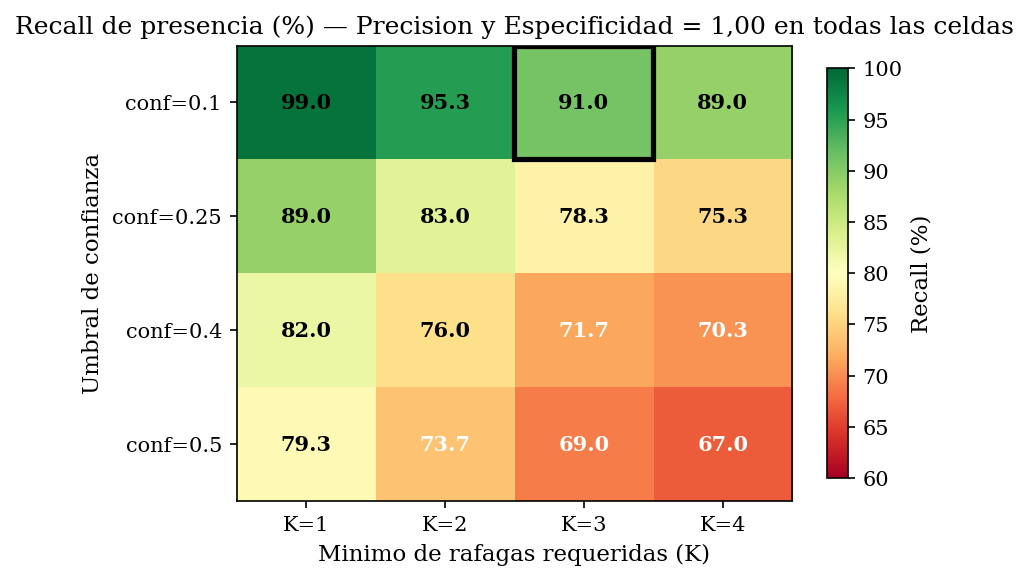
\includegraphics[width=0.70\textwidth]{figuras/resultados/presencia_heatmap.png}
    \caption{Mapa de calor del recall de presencia (\%) en función del umbral de confianza $\mathit{thr}$ y del mínimo de ráfagas~$K$. Las celdas más claras corresponden a mayor recall. El recuadro destacado marca el punto de operación recomendado ($\mathit{thr}=0{,}10$,\, $K=3$), con recall del \SI{91}{\percent} y F1\,=\,\num{0,953}. La precisión y la especificidad valen \num{1,000} en todas las celdas.}
    \label{fig:presencia_heatmap}
\end{figure}

\FloatBarrier
Como punto de operación se adopta $\mathit{thr}=0{,}10$,\, $K=3$, que maximiza el recall de presencia (\SI{91}{\percent}, F1\,=\,\num{0,953}) exigiendo a la vez la coincidencia de tres ráfagas independientes por ventana, lo que protege frente a detecciones espurias aisladas. En este punto, de las \num{300}~ventanas con dron el sistema confirma \num{273} y deja \num{27} sin confirmar (falsos negativos), mientras que las \num{300}~ventanas de interferencia pura se rechazan en su totalidad, sin una sola falsa alarma.


\subsection{Discusión}
\label{sec:p3_discusion}

El resultado central de P3 es la ausencia total de falsos positivos en las \num{16}~configuraciones evaluadas: el sistema no confirma la presencia de un dron en ningún espectrograma que contenga únicamente WiFi y Bluetooth, incluidas las capturas de interferencia más intensa. La precisión y la especificidad perfectas se mantienen con independencia de los parámetros del clasificador de presencia, lo que indica que la decisión positiva del sistema es altamente fiable.


La aparente paradoja entre el recall de caja (\SI{39}{\percent}) y el recall de presencia (\SI{91}{\percent}) se explica por la redundancia temporal del protocolo OcuSync. Una ventana con dron contiene decenas de ráfagas FHSS ---consecuencia directa de un esquema de salto que cambia de canal decenas de veces por cada \SI{0.1}{\second}---, de modo que, aunque el detector falle la mayoría de las ráfagas a nivel individual, le basta con acertar unas pocas para superar el mínimo de $K=3$. El clasificador de presencia actúa así como un agregador que convierte múltiples detecciones débiles en una decisión binaria robusta. En las ventanas sin dron, por el contrario, las detecciones espurias son tan escasas que nunca alcanzan ese mínimo, lo que sostiene la especificidad perfecta.


El análisis por captura matiza el origen de los \num{27}~falsos negativos: se concentran en la captura a \SI{5}{\meter} con WiFi limpio (nivel L1), mientras que la captura a \SI{10}{\meter} con WiFi saturado (nivel L3) se confirma en el \SI{100}{\percent} de sus ventanas. Este comportamiento, contraintuitivo a primera vista, admite una explicación coherente con el protocolo: ante una interferencia intensa, OcuSync tiende a incrementar la densidad de retransmisiones, lo que aumenta el número de ráfagas por ventana y facilita la confirmación de presencia. De ser correcta esta interpretación, el sistema operaría mejor precisamente en el escenario de despliegue más exigente.


Conviene encuadrar el alcance de estas cifras: el barrido se ha realizado sobre el conjunto de prueba del dataset~v3, de carácter interior y controlado (\cref{cap:implementacion}). La especificidad perfecta y el recall del \SI{91}{\percent} son sólidos dentro de ese dominio; su validación sobre un conjunto con mayor diversidad de distancias, niveles de interferencia y entornos ---el dataset~v4 propuesto en el \cref{cap:conclusiones}--- queda planteada como trabajo futuro. En cualquier caso, el punto de operación $\mathit{thr}=0{,}10$,\, $K=3$ constituye un compromiso razonable entre sensibilidad y robustez para una primera versión del sistema de vigilancia.


\section{P4 --- ¿Identifica el sistema el modelo de dron y discrimina por morfología o por intensidad?}
\label{sec:bloque_clasificacion}

Esta sección responde a dos preguntas relacionadas: si el clasificador ResNet18 puede identificar el modelo concreto de dron una vez confirmada la presencia, y si la discriminación aprendida se sustenta en la morfología espectro-temporal de las ráfagas o en el nivel medio de potencia. La primera evalúa la segunda etapa del \emph{pipeline}; la segunda cierra la hipótesis central del trabajo.

\subsection{Planteamiento del experimento}
\label{sec:p4_planteamiento}

\paragraph{Parte A --- Clasificación de modelos.}
El clasificador Stage~2, cuya arquitectura y configuración de entrenamiento se describen en la \cref{sec:implementacion_stage2}, distingue seis clases: cinco modelos de plataforma (\emph{f450}, \emph{hunter}, \emph{mavic\_video}, \emph{mavic\_novideo} y \emph{mini3}) más la clase \emph{interference}, a partir de capturas de campo abierto con drones reales. El conjunto de prueba contiene \num{941}~segmentos de \num{8}~capturas distintas, particionados por captura. El mejor modelo, seleccionado por macro-F1 sobre validación, corresponde a la época~\num{10} (macro-F1 de validación \num{0,959}).

El Mavic se separa en dos clases ---\emph{mavic\_video} y \emph{mavic\_novideo}--- porque durante la captura se recorrió todo el espectro en busca de la señal del dron. Esto dio lugar a dos tipos de región según el instante: tramos en los que el enlace transmitía vídeo (canal OFDM de banda ancha) y tramos en los que solo emitía la señal de control FHSS. Ambas condiciones presentan una morfología distinta en el espectrograma, por lo que se etiquetan como clases separadas.

\paragraph{Parte B --- Barrido de SNR.}
Para verificar si la clasificación se apoya en la morfología o en el nivel de energía se emplea el protocolo de barrido descrito en la \cref{sec:implementacion_snr}: se inyectan dos tipos de ruido (AWGN y FHSS sintético) a la misma potencia total en el dominio IQ, y se regenera el espectrograma con el mismo \emph{pipeline} de entrenamiento. El barrido cubre los niveles de SNR $\{+\infty,\, +20,\, +15,\, +10,\, +5,\, 0,\, -5,\, -10,\, -15,\, -20\}$~dB.

La hipótesis es que, si el clasificador discrimina por morfología --- por \emph{dónde} está la energía, no por \emph{cuánta} hay ---, el FHSS sintético (que concentra toda su potencia en el \SI{1,5}{\percent} del plano tiempo-frecuencia) debería degradar el rendimiento mucho menos que el AWGN (que distribuye esa misma potencia uniformemente por toda la imagen).

\subsection{Resultados de clasificación multiclase}
\label{sec:p4_clasificacion}

La \cref{fig:stage2_curvas} muestra la evolución de la pérdida y el macro-F1 del clasificador durante el entrenamiento. El \textbf{macro-F1} es la media aritmética del F1 de las seis clases, dando a cada una el mismo peso con independencia de su número de muestras; por ello penaliza con fuerza el fallo en una clase minoritaria, lo que lo convierte en una métrica exigente y adecuada para un conjunto desbalanceado como este.

\begin{figure}[htbp]
    \centering
    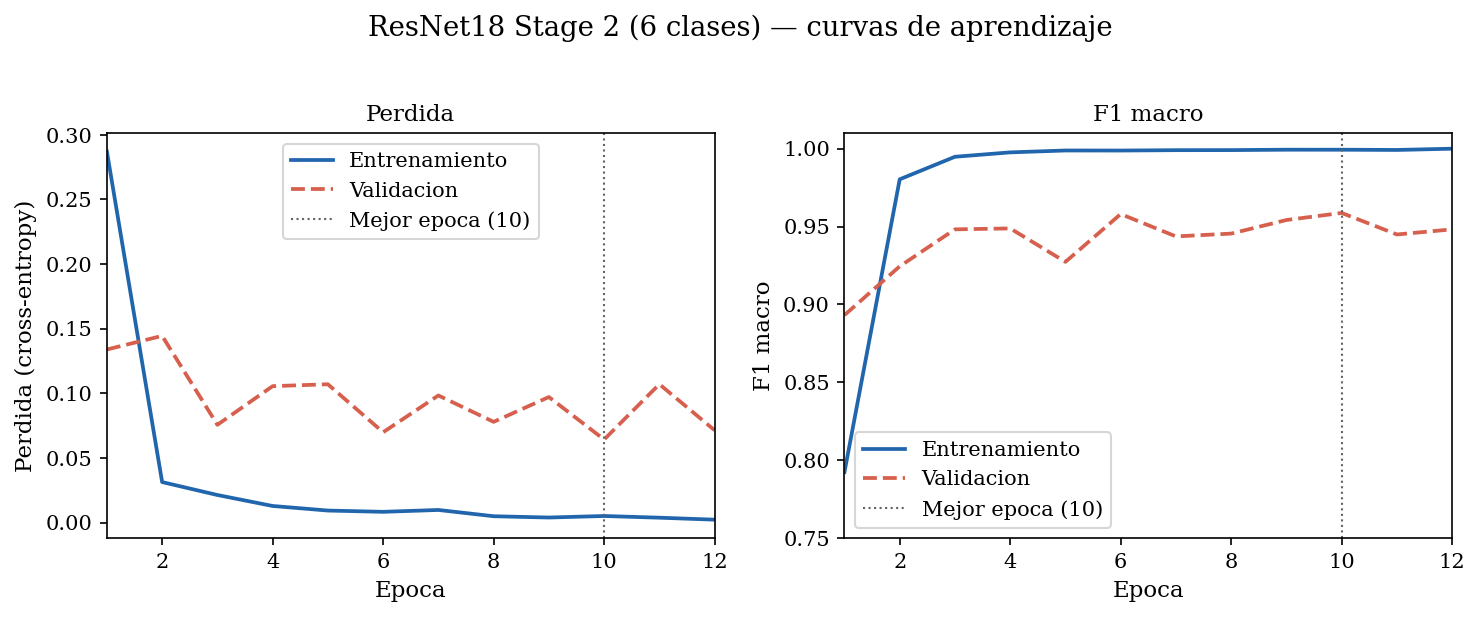
\includegraphics[width=0.85\textwidth]{figuras/resultados/stage2_curvas_aprendizaje.png}
    \caption{Evolución de la pérdida y el macro-F1 en entrenamiento y validación del clasificador ResNet18 de seis clases. El macro-F1 promedia el F1 de las seis clases con igual peso. La curva de entrenamiento asciende hacia F1\,=\,1,0, mientras que la de validación oscila entre \num{0,93} y \num{0,96}. Esta brecha indica sobreajuste moderado y justifica seleccionar el \emph{checkpoint} de mejor macro-F1 en validación en lugar de la última época.}
    \label{fig:stage2_curvas}
\end{figure}

Las curvas muestran un sobreajuste moderado: el F1 de entrenamiento sube hacia \num{1,0} mientras que el de validación oscila sin convergencia clara al final del entrenamiento. Esto justifica haber seleccionado el \emph{checkpoint} de la época~\num{10} por su máximo F1 de validación.
Los resultados globales sobre el conjunto de prueba se presentan en la \cref{tab:stage2_global}. El resultado más relevante para este TFG es que el DJI Mini~3 obtiene F1\,=\,\num{0,992} sobre \num{300}~muestras: prácticamente clasificación sin errores. Las clases \emph{mavic\_video} y \emph{f450} también se reconocen con alta fiabilidad.

\begin{table}[htbp]
\centering
\caption{Resultados globales del clasificador ResNet18 de seis clases sobre el conjunto de prueba (\num{941}~segmentos).}
\label{tab:stage2_global}
\begin{tabular}{lc}
\toprule
\textbf{Métrica} & \textbf{Valor} \\
\midrule
Exactitud       & 0,898 \\
F1~macro        & 0,764 \\
F1~ponderado    & 0,872 \\
Precisión macro & 0,730 \\
Recall macro    & 0,819 \\
\bottomrule
\end{tabular}
\end{table}

El desglose por clase de la \cref{tab:stage2_por_clase} localiza el origen del macro-F1 de \num{0,764}: está íntegramente condicionado por el rendimiento de una única clase.

\begin{table}[htbp]
\centering
\caption{Métricas por clase del clasificador ResNet18 de seis clases sobre el conjunto de prueba.}
\label{tab:stage2_por_clase}
\begin{tabular}{lcccc}
\toprule
\textbf{Clase}       & \textbf{Soporte} & \textbf{Precisión} & \textbf{Recall} & \textbf{F1} \\
\midrule
f450                 & 30               & 0,811              & 1,000           & 0,896 \\
hunter               & 120              & 0,588              & 1,000           & 0,741 \\
mavic\_video         & 120              & 1,000              & 1,000           & 1,000 \\
mavic\_novideo       & 71               & 0,000              & 0,000           & 0,000 \\
mini3                & 300              & 0,984              & 1,000           & 0,992 \\
interference         & 300              & 1,000              & 0,917           & 0,957 \\
\midrule
\textbf{Macro}       & 941              & 0,730              & 0,819           & 0,764 \\
\bottomrule
\end{tabular}
\end{table}

La \cref{fig:stage2_confusion} muestra la distribución de errores mediante la matriz de confusión normalizada. En esta representación las filas corresponden a las clases reales y las columnas a las predichas; los valores de la diagonal indican la proporción de muestras clasificadas correctamente para cada clase, y los valores fuera de la diagonal reflejan las confusiones entre clases.

\begin{figure}[htbp]
    \centering
    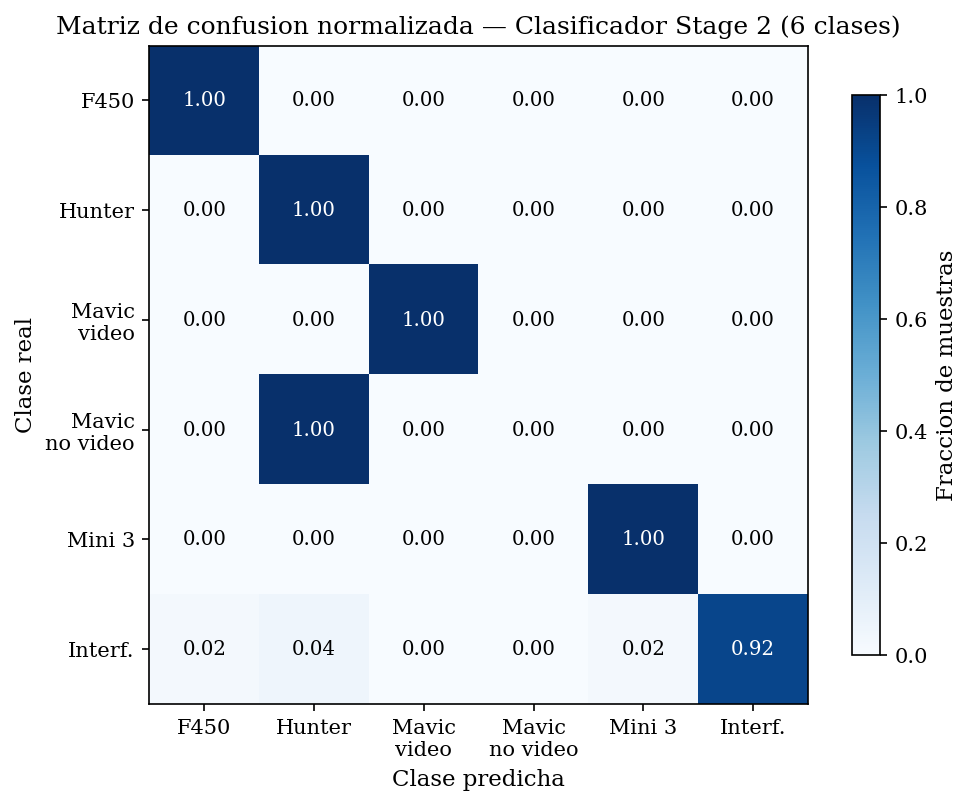
\includegraphics[width=0.75\textwidth]{figuras/resultados/stage2_confusion_matrix_norm.png}
    \caption{Matriz de confusión normalizada del clasificador ResNet18 de seis clases sobre el conjunto de prueba. La diagonal es prácticamente perfecta para cinco clases. La clase \emph{mavic\_novideo} colapsa íntegramente a \emph{hunter}, constituyendo el único fallo relevante del clasificador.}
    \label{fig:stage2_confusion}
\end{figure}




\begin{figure}[htbp]
    \centering
    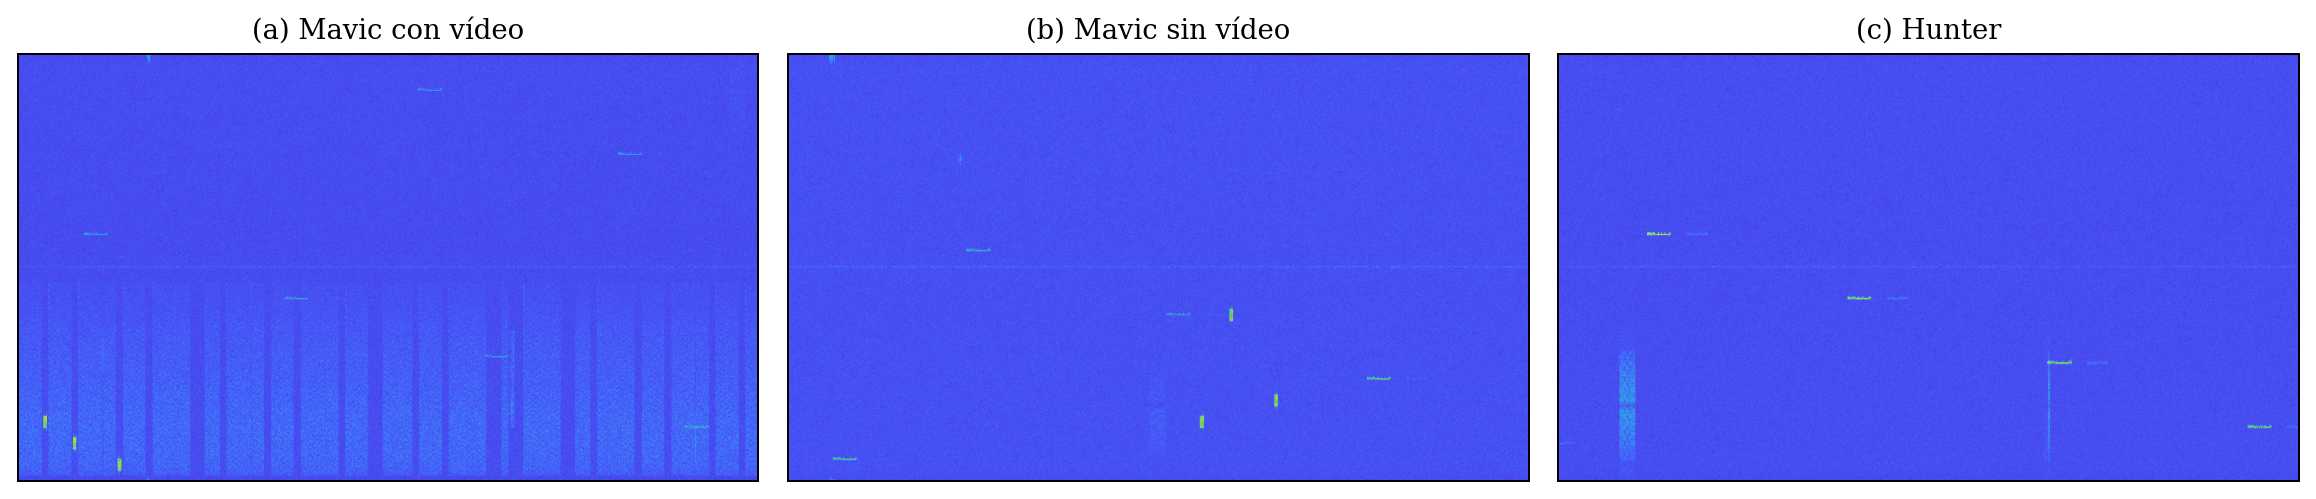
\includegraphics[width=\textwidth]{figuras/resultados/stage2_morfologia_mavic_hunter.png}
    \caption{Comparativa morfológica que explica la confusión entre \emph{mavic\_novideo} y \emph{hunter}. (a) Mavic con vídeo: el enlace emite el canal de banda ancha (OFDM) junto a la señal de control, produciendo bandas anchas y densas claramente distintivas. (b) Mavic sin vídeo: al desactivarse el vídeo, solo queda la señal de control FHSS, reducida a ráfagas dispersas. (c) Hunter: su emisión presenta el mismo aspecto de ráfagas dispersas. Los paneles (b) y (c) son morfológicamente casi indistinguibles, lo que justifica que el clasificador asigne las muestras de \emph{mavic\_novideo} a \emph{hunter}.}
    \label{fig:stage2_morfologia}
\end{figure}



El caso de \emph{mavic\_novideo} no es un fallo metodológico, sino una consecuencia directa de la morfología de la señal, ilustrada en la \cref{fig:stage2_morfologia}. Con el vídeo activo (\cref{fig:stage2_morfologia}a), el Mavic emite un canal OFDM de banda ancha que lo hace inconfundible. Al desactivar el vídeo (\cref{fig:stage2_morfologia}b), su emisión se reduce a la señal de control FHSS ---ráfagas dispersas--- cuya morfología coincide con la del Hunter (\cref{fig:stage2_morfologia}c). Sin el canal de vídeo no queda ningún rasgo espectral que separe ambas clases con los datos disponibles, por lo que el clasificador asigna la totalidad de las muestras de \emph{mavic\_novideo} a \emph{hunter}. Su resolución requeriría más capturas de esta clase en condiciones variadas, no un rediseño del sistema.








\subsection{Resultados del barrido de SNR}
\label{sec:resultados_snr}

La \cref{tab:snr_accuracy} presenta la exactitud del clasificador frente al SNR para ambos modelos de ruido. El control a SNR infinito reproduce exactamente la exactitud del test original (\num{0,898}), confirmando la fidelidad del \emph{pipeline} de inyección al proceso de entrenamiento.



Antes de cuantificar el efecto del ruido conviene observarlo directamente. La \cref{fig:snr_ejemplos} muestra un mismo espectrograma del DJI Mini~3 degradado por los dos modelos de ruido a distintos niveles de SNR: el AWGN (\cref{fig:snr_ejemplo_awgn}) enmascara la señal subiendo el fondo de forma uniforme, mientras que el FHSS sintético (\cref{fig:snr_ejemplo_fhss}) mantiene las ráfagas visibles porque concentra su energía en regiones puntuales. Este contraste anticipa el resultado cuantitativo que se presenta a continuación.



\begin{figure}[htbp]
    \centering
    \begin{subfigure}[b]{\textwidth}
        \centering
        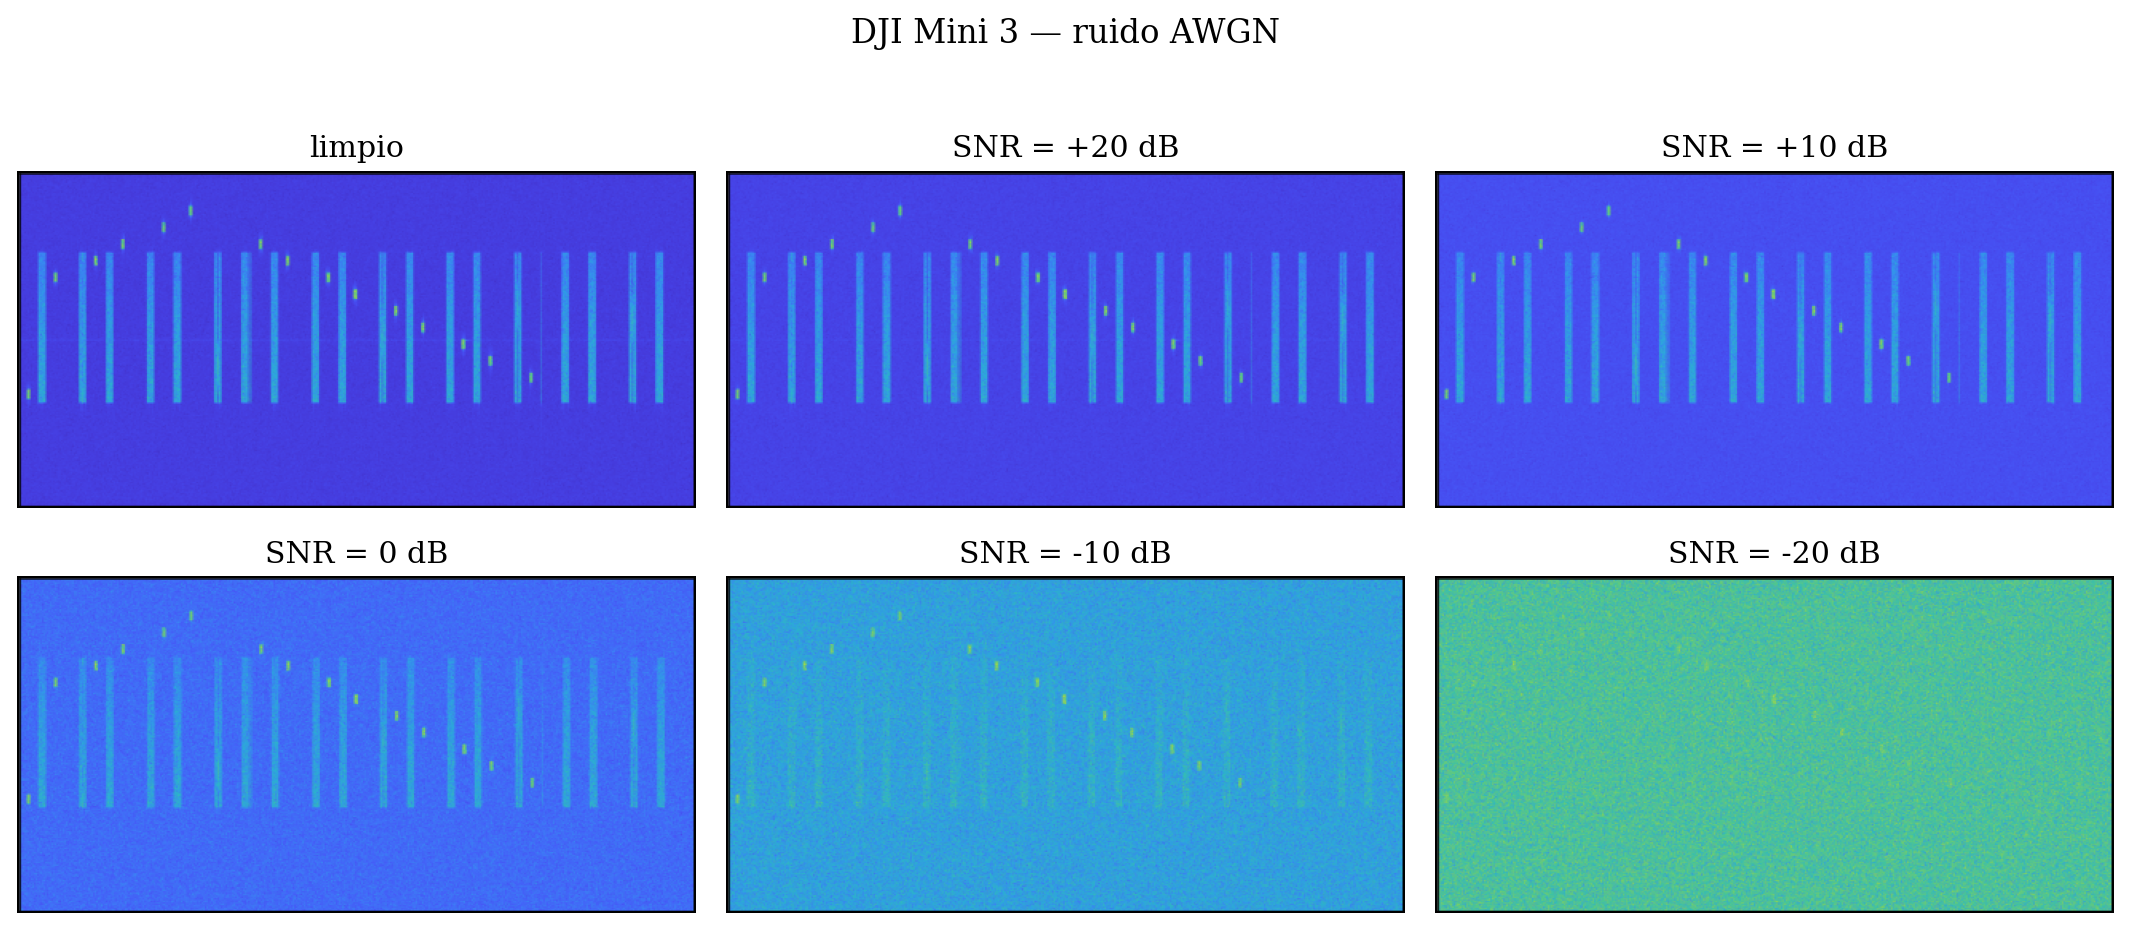
\includegraphics[width=\textwidth]{figuras/resultados/snr_ejemplo_mini3_awgn.png}
        \caption{Ruido AWGN: la energía se reparte por todo el plano. Al bajar el SNR, el fondo sube de forma uniforme hasta enmascarar por completo las ráfagas (a $-20$~dB la firma es inapreciable).}
        \label{fig:snr_ejemplo_awgn}
    \end{subfigure}

    \vspace{0.4em}

    \begin{subfigure}[b]{\textwidth}
        \centering
        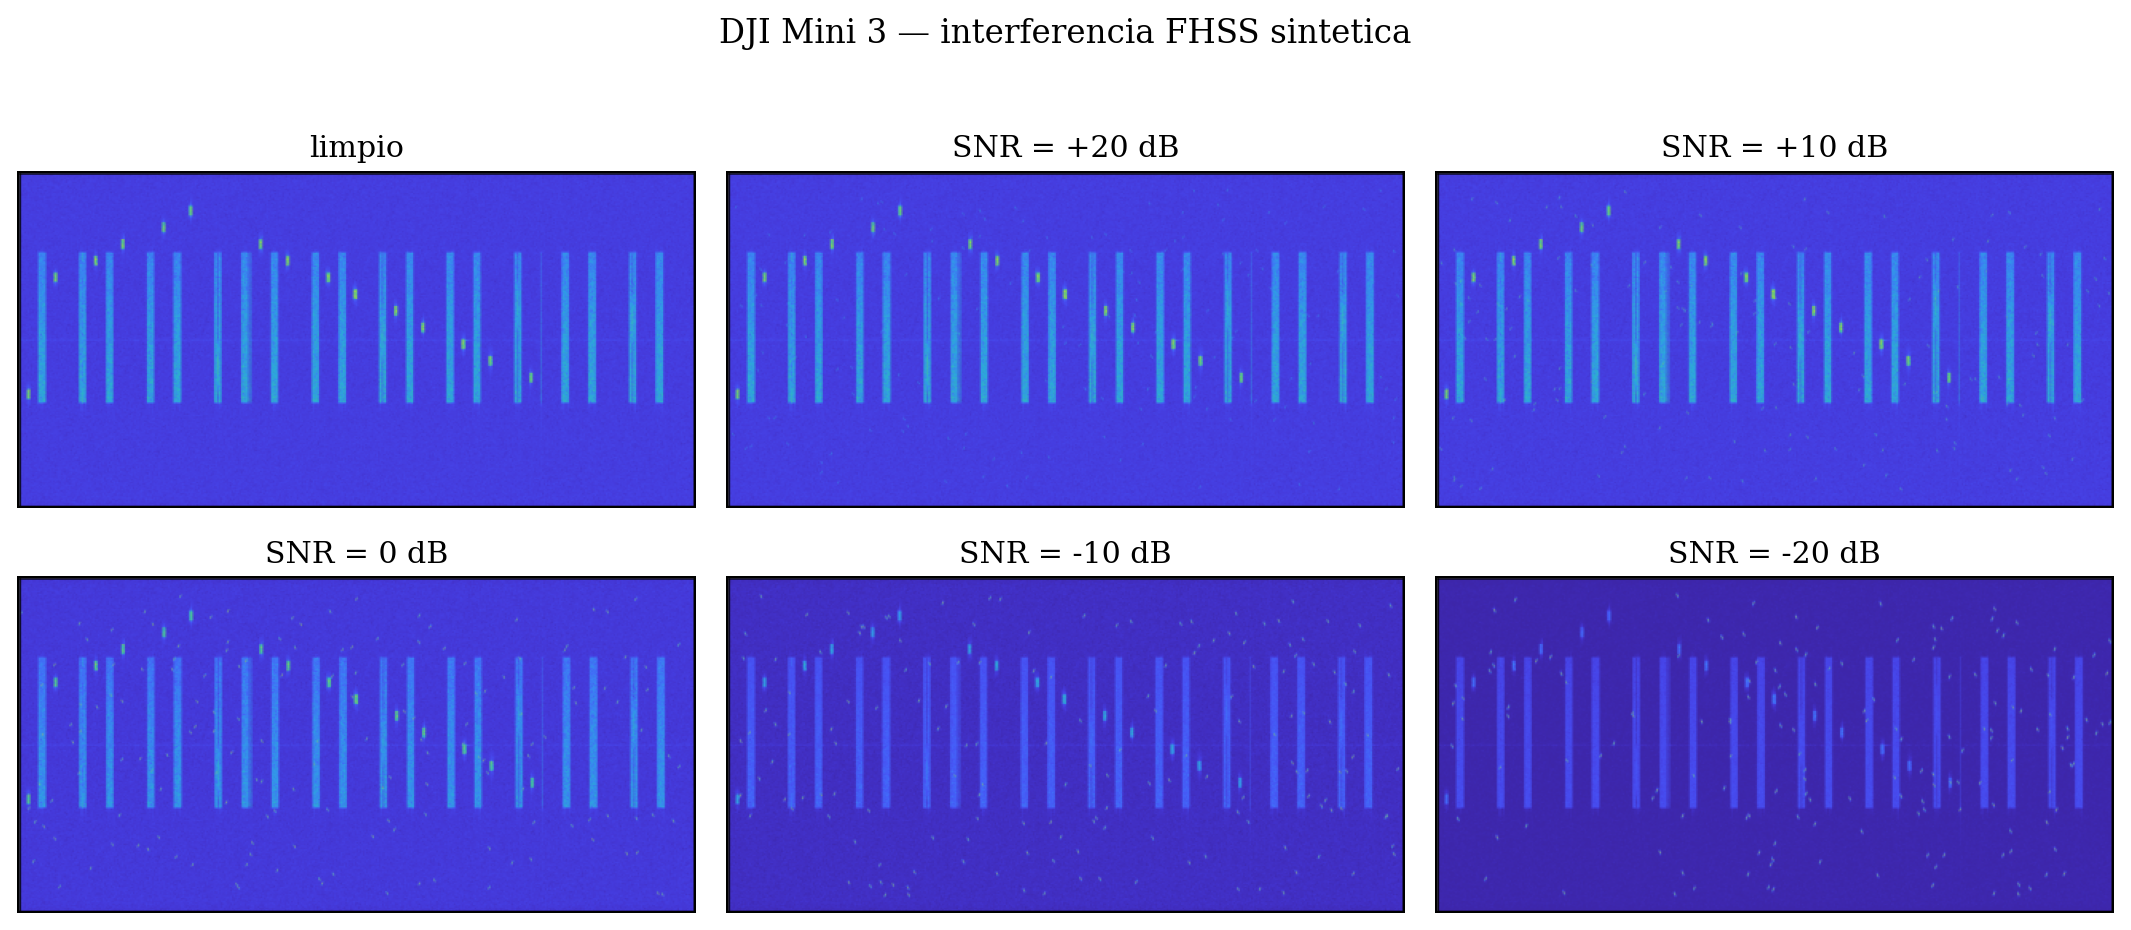
\includegraphics[width=\textwidth]{figuras/resultados/snr_ejemplo_mini3_fhss.png}
        \caption{Interferencia FHSS sintética: la energía se concentra en ráfagas puntuales. El fondo apenas cambia y las ráfagas de OcuSync del Mini~3 siguen siendo visibles incluso a SNR muy bajo.}
        \label{fig:snr_ejemplo_fhss}
    \end{subfigure}
    \caption{Efecto de los dos modelos de ruido sobre un espectrograma del DJI Mini~3 a distintos niveles de SNR, con la misma potencia total inyectada. El AWGN (a) destruye la firma espectral al subir el fondo de forma homogénea, mientras que el FHSS (b) deja intacto el \SI{98,5}{\percent} del plano tiempo-frecuencia y preserva la morfología de las ráfagas. Esta diferencia explica visualmente por qué el clasificador resiste mucho mejor el ruido FHSS.}
    \label{fig:snr_ejemplos}
\end{figure}



\begin{table}[htbp]
\centering
\caption{Exactitud del clasificador de seis clases frente al SNR para ruido AWGN e interferencia FHSS sintética.}
\label{tab:snr_accuracy}
\begin{tabular}{lcc}
\toprule
\textbf{SNR (dB)} & \textbf{AWGN} & \textbf{FHSS} \\
\midrule
$+\infty$ & 0,898 & 0,898 \\
$+20$     & 0,900 & 0,899 \\
$+10$     & 0,889 & 0,899 \\
$+5$      & 0,848 & 0,908 \\
$0$       & 0,691 & 0,912 \\
$-5$      & 0,239 & 0,852 \\
$-10$     & 0,136 & 0,748 \\
$-15$     & 0,133 & 0,676 \\
$-20$     & 0,133 & 0,557 \\
\bottomrule
\end{tabular}
\end{table}

La \cref{fig:snr_accuracy} representa gráficamente las dos curvas de exactitud frente al SNR.

\begin{figure}[htbp]
    \centering
    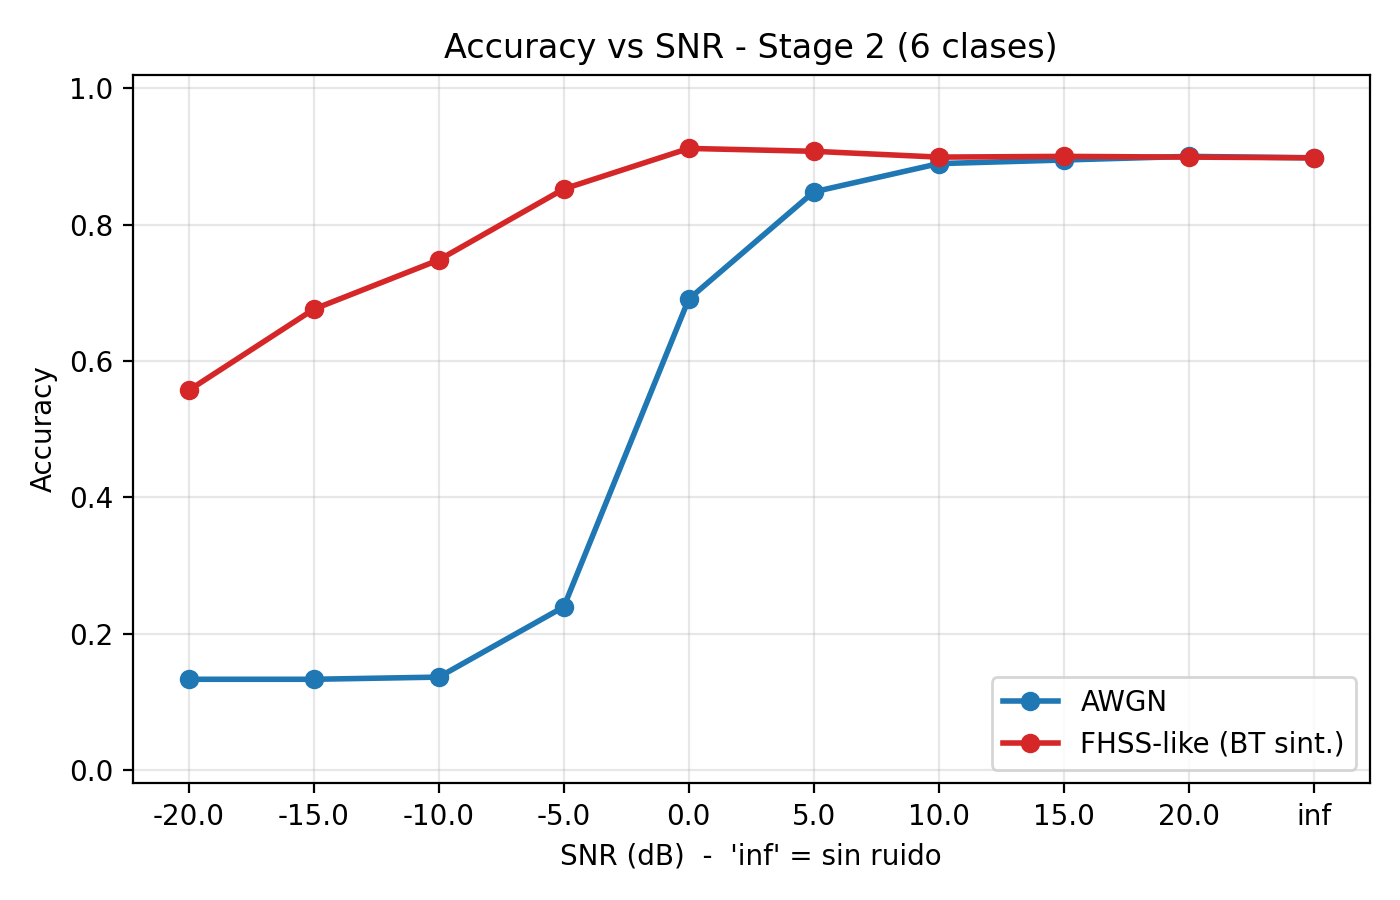
\includegraphics[width=0.85\textwidth]{figuras/resultados/snr_accuracy_vs_snr.png}
    \caption{Exactitud del clasificador frente al SNR para AWGN (azul) y FHSS sintético (naranja). El AWGN presenta un codo brusco entre $+5$~dB y $-5$~dB, con exactitud cayendo de \num{0,848} a \num{0,239}. El FHSS sintético mantiene exactitud superior a \num{0,85} hasta $-5$~dB y superior a \num{0,55} a $-20$~dB. La diferencia máxima entre ambas curvas, de \num{0,61}~puntos de exactitud, se alcanza a $-5$~dB.}
    \label{fig:snr_accuracy}
\end{figure}

La \cref{fig:snr_f1macro} muestra la evolución del macro-F1, que al tratar todas las clases por igual permite evaluar el impacto del ruido de forma independiente del desbalanceo entre clases.

\begin{figure}[htbp]
    \centering
    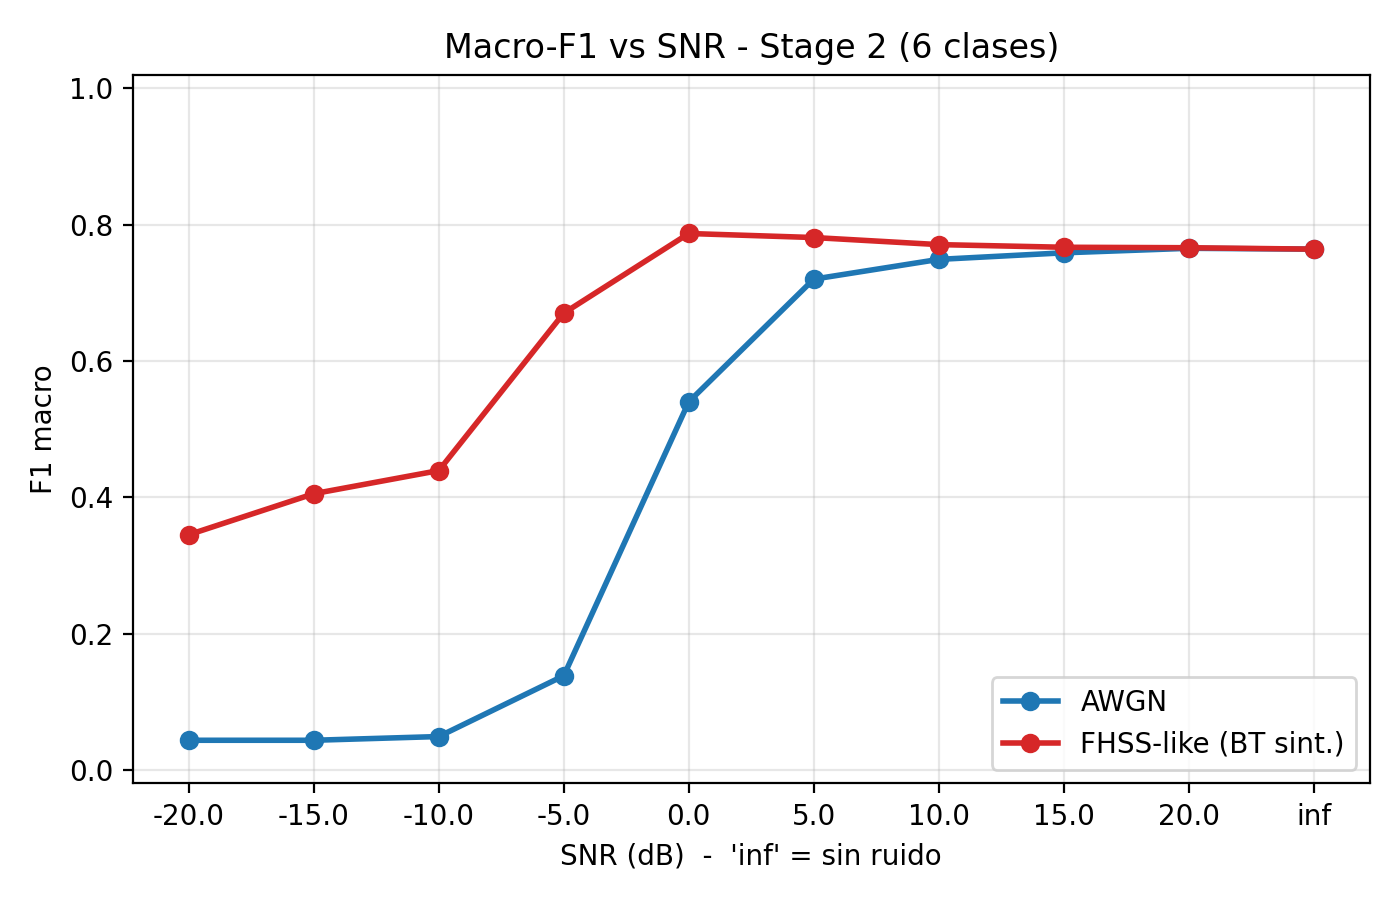
\includegraphics[width=0.85\textwidth]{figuras/resultados/snr_f1_macro_vs_snr.png}
    \caption{Macro-F1 del clasificador frente al SNR para ambos modelos de ruido. La tendencia es análoga a la de la exactitud: el AWGN produce una degradación notablemente más abrupta que el FHSS sintético.}
    \label{fig:snr_f1macro}
\end{figure}

La \cref{fig:snr_panel} muestra las matrices de confusión del clasificador a cuatro niveles de SNR representativos, para ambos modelos de ruido.

\begin{figure}[htbp]
    \centering
    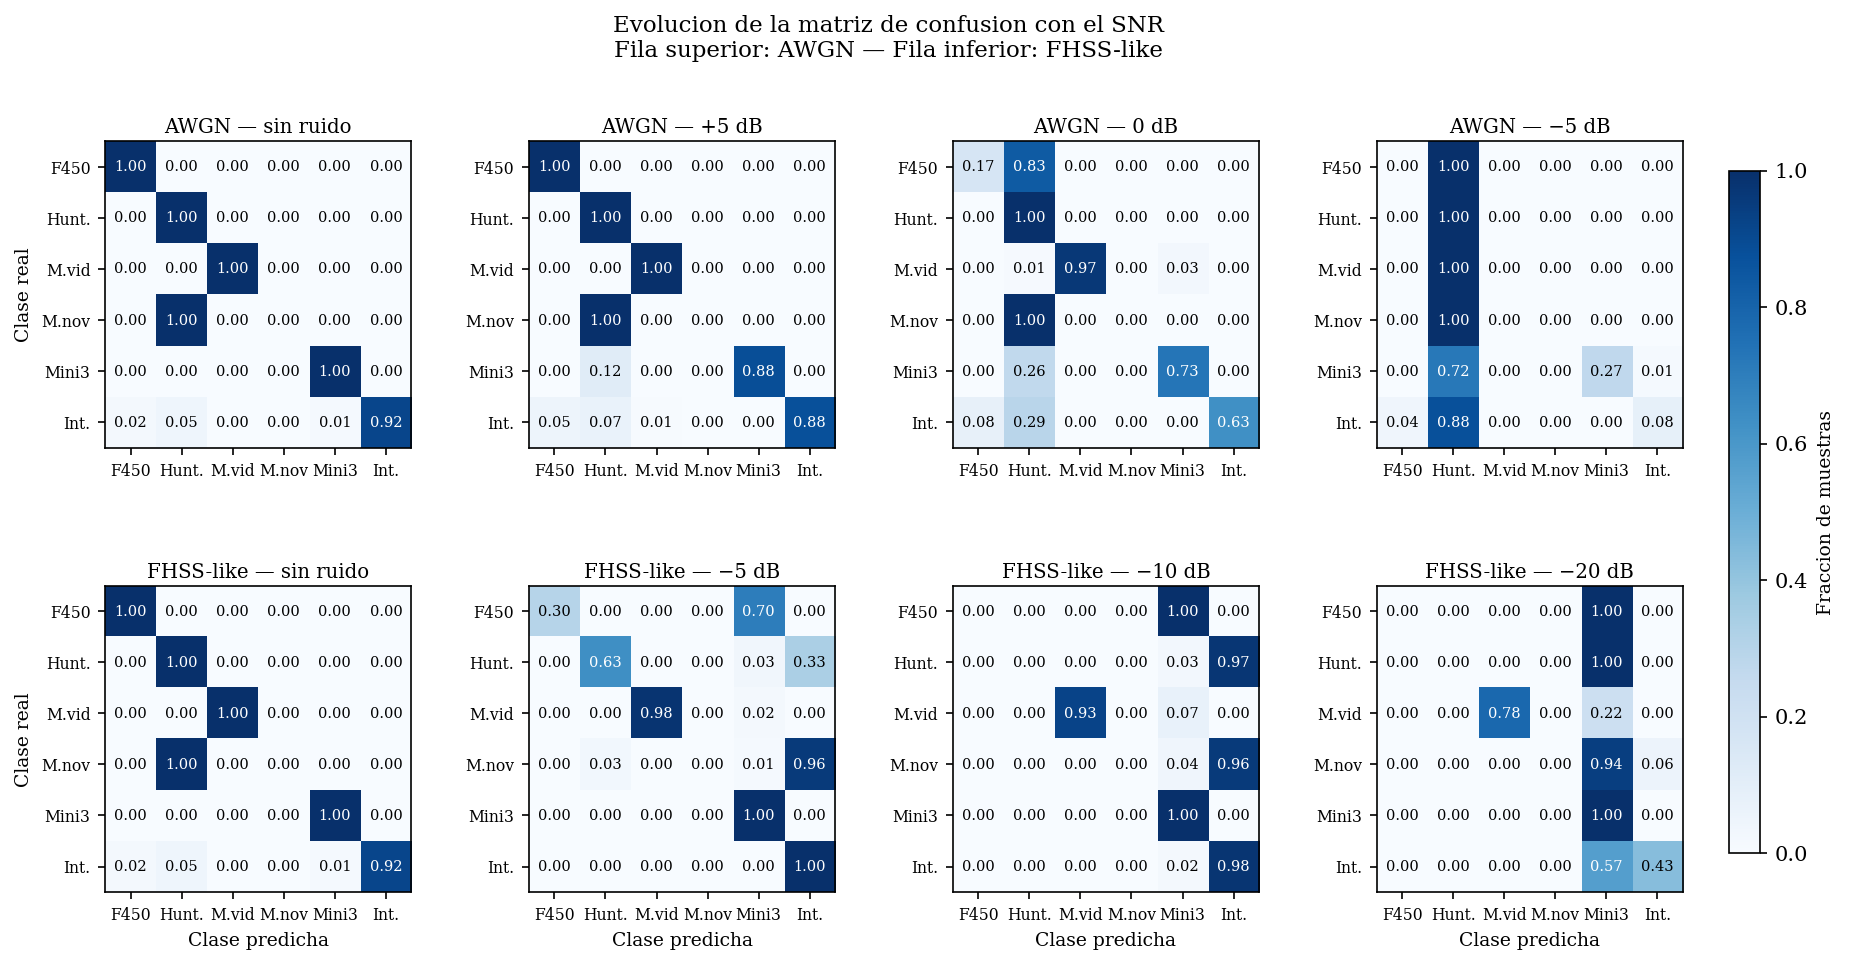
\includegraphics[width=\textwidth]{figuras/resultados/snr_confusion_panel.png}
    \caption{Panel de matrices de confusión del clasificador de seis clases a distintos niveles de SNR, para ruido AWGN (fila superior) y FHSS sintético (fila inferior). El AWGN dispersa las predicciones hacia clases incorrectas conforme decrece el SNR; el FHSS sintético mantiene la diagonal prácticamente intacta hasta $-5$~dB.}
    \label{fig:snr_panel}
\end{figure}

Las matrices del panel muestran que, bajo AWGN, la degradación es difusa: las predicciones se distribuyen hacia múltiples clases incorrectas conforme baja el SNR. Bajo FHSS sintético, en cambio, la diagonal se mantiene coherente hasta $-5$~dB y solo se degrada de forma apreciable a partir de $-10$~dB.

% =============================================================================
\subsection{Discusión}
\label{sec:p4_discusion}

\paragraph{Identificación del modelo de dron.}
La primera parte de P4 confirma que el sistema no solo detecta la presencia de un dron, sino que identifica su modelo concreto. El DJI Mini~3 ---la plataforma objetivo de este trabajo--- se clasifica correctamente en prácticamente la totalidad de las muestras (F1\,=\,\num{0,992}), y la clase \emph{interference} obtiene precisión \num{1,000}: ninguna señal real de interferencia se confunde de forma sistemática con un dron, en línea con la ausencia de confusión cruzada observada en P2 y P3. Los \num{25}~errores sobre \num{300}~muestras de interferencia se reparten entre varias clases de dron sin concentrarse en ninguna, lo que descarta un sesgo sistemático.

El único fallo relevante ---el colapso de \emph{mavic\_novideo} sobre \emph{hunter}--- no contradice la hipótesis central del trabajo, sino que la refuerza. Como muestra la \cref{fig:stage2_morfologia}, cuando el Mavic deja de transmitir vídeo su emisión se reduce a la señal de control FHSS, morfológicamente indistinguible de la del Hunter. Que el clasificador agrupe ambas clases es precisamente lo que cabe esperar de una red que decide por la \emph{forma} de la señal y no por una etiqueta o por el contexto de captura: ante dos morfologías idénticas, emite la misma predicción. El error no es, por tanto, un defecto del modelo, sino una limitación de los datos ---la ausencia, en ese modo de emisión, de cualquier rasgo espectral que separe las dos plataformas---, resoluble con más capturas de la clase en condiciones variadas y no con un rediseño del sistema.

\paragraph{Cómo se inyecta el ruido.}
Conviene recordar cómo se construyen ambos ruidos, descritos en detalle en la \cref{sec:implementacion_snr}, porque su forma de generación es la clave de la comparación. Los dos se inyectan en el dominio IQ complejo de la señal y se calibran a la \emph{misma potencia total} para cada SNR objetivo, de modo que la única variable que cambia entre ellos es cómo se reparte esa energía en el plano tiempo-frecuencia. 

El \textbf{ruido blanco AWGN} es ruido gaussiano complejo, $n[k]\sim\mathcal{CN}(0,\sigma^2)$, sumado muestra a muestra a la señal con la varianza $\sigma^2$ ajustada al SNR objetivo; al ser blanco, su energía se distribuye de forma uniforme por toda la banda y toda la ventana, elevando el fondo del espectrograma por igual en todo el plano. 

El \textbf{ruido FHSS sintético} emula una interferencia tipo Bluetooth Classic: genera unas \num{160}~ráfagas por ventana de \SI{0.1}{\second} (\num{1600}~saltos/s), cada una de \SI{366}{\micro\second} de duración y aproximadamente \SI{1}{\mega\hertz} de ancho, colocada en un instante y una frecuencia aleatorios dentro de la banda capturada y suavizada con una ventana de Hann. Como el conjunto se calibra a la misma potencia total que el AWGN, esa energía idéntica queda concentrada en rectángulos estrechos y dispersos ---morfológicamente parecidos a las propias ráfagas del dron--- que ocupan solo en torno al \SI{1,5}{\percent} del plano tiempo-frecuencia.

\paragraph{Robustez frente al ruido.}
La segunda parte de P4 somete al clasificador a dos modelos de ruido de la misma potencia total pero distinta distribución en el plano tiempo-frecuencia. El contraste es nítido tanto a nivel visual como cuantitativo. Visualmente (\cref{fig:snr_ejemplos}), el AWGN eleva el fondo de forma uniforme hasta enmascarar por completo las ráfagas a $-20$~dB, mientras que el FHSS sintético deja intacto el grueso del espectrograma y mantiene visibles las ráfagas de OcuSync incluso a SNR muy bajo. Cuantitativamente, esa diferencia se traduce en el codo abrupto del AWGN entre $+5$ y $-5$~dB ---una caída de \num{0,61}~puntos de exactitud--- frente a la degradación suave del FHSS, que conserva una exactitud superior a \num{0,85} hasta $-5$~dB.

Esta asimetría solo admite una explicación: la red discrimina por \emph{dónde} está la energía, no por \emph{cuánta} hay. El AWGN reparte su potencia por los \SI{40}{\mega\hertz} del espectrograma y, al superar el nivel de la señal, borra la firma de las ráfagas; el FHSS sintético concentra la misma potencia en aproximadamente el \SI{1,5}{\percent} del plano, de modo que el \SI{98,5}{\percent} restante ---y con él la morfología del dron--- permanece intacto. Si el clasificador se apoyase en el nivel medio de potencia, ambos ruidos lo degradarían por igual, dado que inyectan la misma energía total; que el AWGN sea mucho más destructivo demuestra lo contrario.

\paragraph{Síntesis: la red discrimina por morfología.}
Las dos partes de P4 convergen en la misma conclusión y cierran la hipótesis central del trabajo. La confusión \emph{mavic\_novideo}--\emph{hunter} muestra que la red agrupa señales por su morfología espectro-temporal; el barrido de SNR muestra que su decisión sobrevive mientras esa morfología sea visible y se desploma solo cuando el ruido la borra. Ambas observaciones son coherentes con los mapas de GradCAM del experimento P1 y de EigenCAM del experimento P2, donde las activaciones de la red se localizaban sobre las estructuras de ráfaga y no sobre el fondo. El clasificador no aprende la intensidad media de la captura ni un atajo contextual, sino la posición de la energía en el plano tiempo-frecuencia: la firma morfológica del dron. Este resultado, sólido para el DJI Mini~3 sobre el conjunto de prueba, sustenta la tesis del trabajo, con la cautela de que su validación en condiciones de despliegue más diversas queda planteada como línea futura.
% =============================================================================


\section{Detección de otros drones no vistos en el entrenamiento}
\label{sec:zeroshot}

Hasta aquí el detector se ha entrenado y evaluado únicamente con el DJI Mini~3. Surge entonces una pregunta natural: ¿lo que ha aprendido sirve para otros drones, o solo sabe reconocer al Mini~3? Para responderla se hace una prueba directa: se toma el detector ya entrenado, \emph{sin reentrenarlo ni ajustar nada}, y se le pasan espectrogramas de tres drones que nunca participaron en el entrenamiento ---un DJI~F450, un Mavic~Pro y un Hunter---, capturados al aire libre. Si el detector es capaz de localizar las ráfagas de estos drones desconocidos, será señal de que ha aprendido a reconocer la \emph{forma} de una transmisión FHSS en general, y no la firma concreta del Mini~3.

La distinción tiene una consecuencia práctica importante. Un lector de paquetes convencional necesitaría conocer y decodificar el protocolo de enlace de cada modelo de dron; en cambio, un detector que reconoce la forma de la señal funciona con cualquier dron que transmita de manera parecida, aunque emplee otro protocolo o una frecuencia distinta. Los tres drones de la prueba transmiten además en frecuencias centrales separadas entre \SI{30}{\mega\hertz} y \SI{50}{\mega\hertz} de la del entrenamiento, de modo que la prueba mide también si el detector depende de la posición absoluta en frecuencia.

\subsection{Cómo detecta las ráfagas de cada dron}
\label{sec:zeroshot_ejemplos}

La \cref{fig:zeroshot_comparativa} muestra la respuesta del detector ante un espectrograma representativo de cada plataforma. En el F450 y el Mavic~Pro el detector dibuja cajas rojas ---predicción \emph{drone}--- justo sobre las ráfagas FHSS, exactamente igual que hacía con el Mini~3, a pesar de no haberlos visto nunca durante el entrenamiento. En el Hunter, en cambio, no dibuja ninguna caja de dron.

\begin{figure}[htbp]
    \centering
    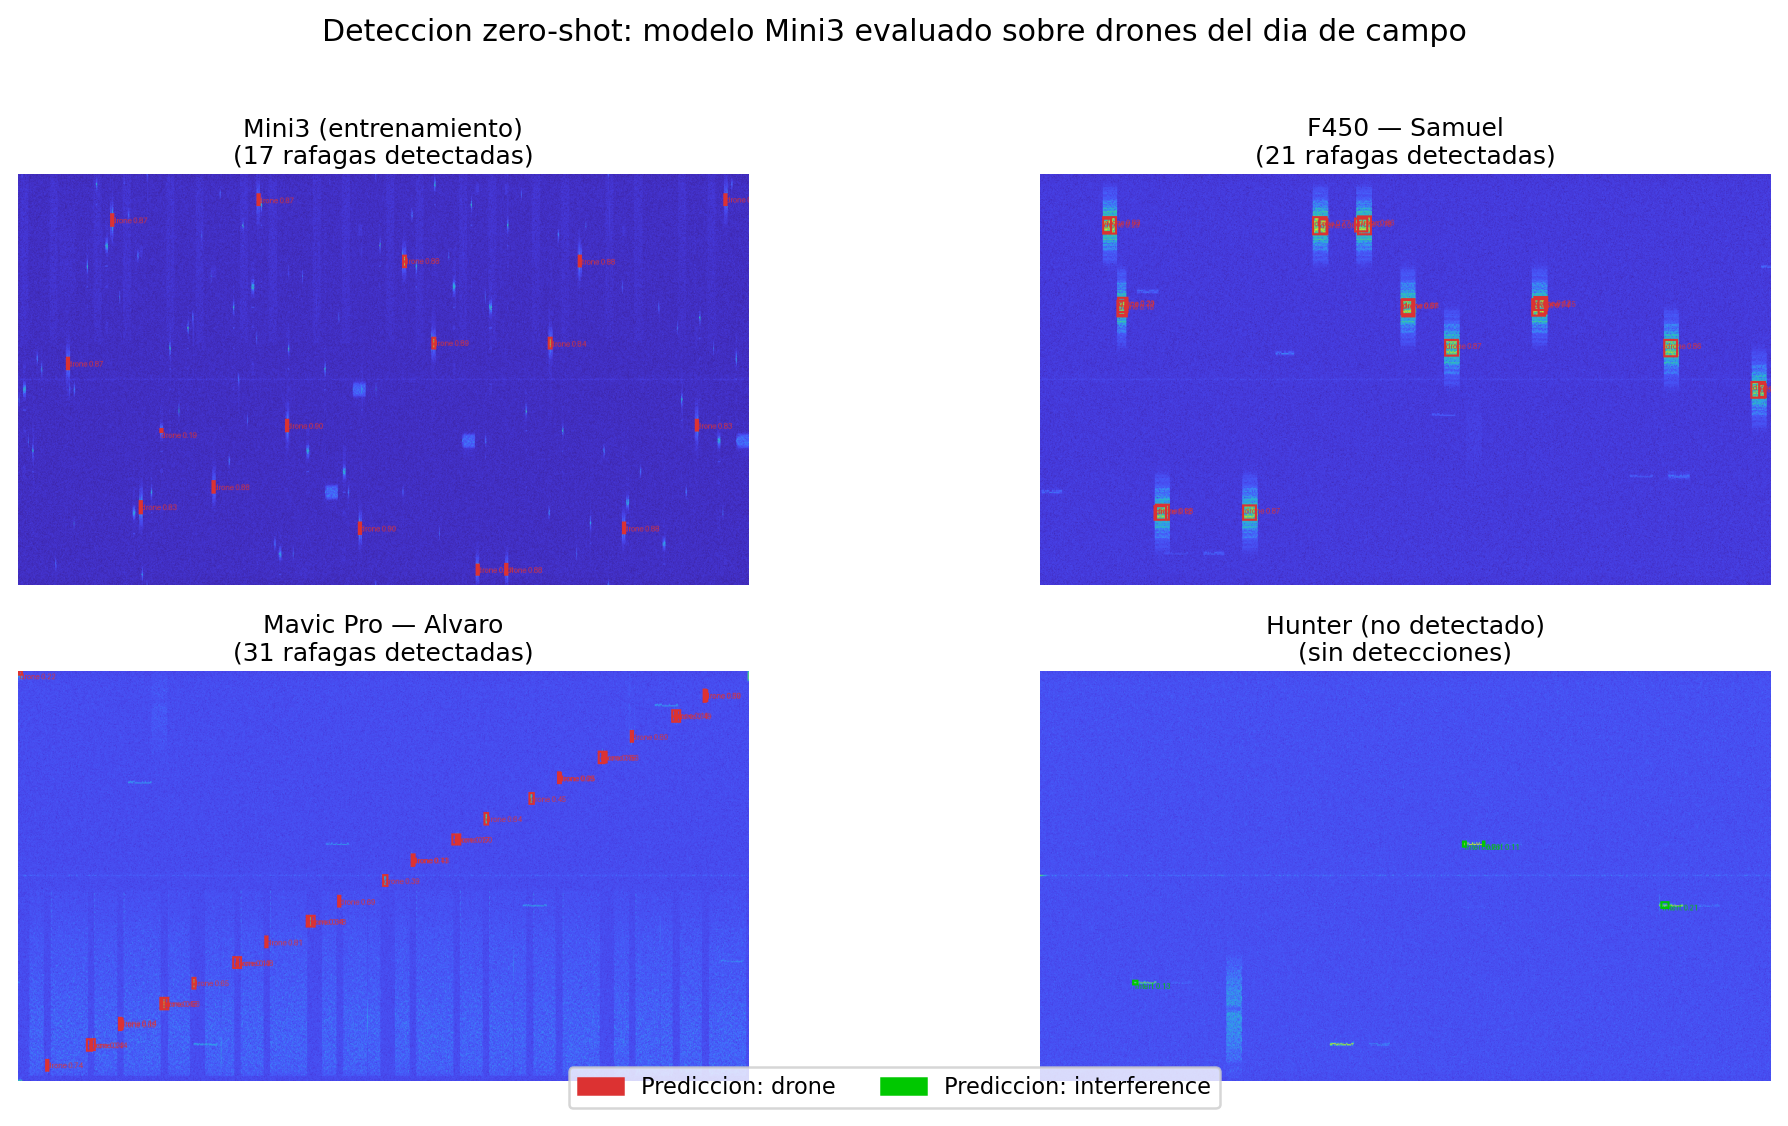
\includegraphics[width=\textwidth]{figuras/resultados/zeroshot_comparativa.png}
    \caption{Detección sobre drones no vistos en el entrenamiento. Para cada plataforma se muestra un espectrograma con las predicciones del detector superpuestas (rojo: \emph{drone}; verde: \emph{interference}). En el Mini~3 (referencia), el F450 y el Mavic~Pro el detector marca en rojo las ráfagas FHSS. En el Hunter no emite ninguna caja de dron, porque su señal no presenta esa morfología.}
    \label{fig:zeroshot_comparativa}
\end{figure}

\FloatBarrier
\subsection{Estadísticas: cuántas ráfagas detecta en cada dron}
\label{sec:zeroshot_estadisticas}

Para cuantificar el comportamiento basta con contar, de media, cuántas ráfagas de dron detecta en cada imagen y en qué porcentaje de imágenes confirma la presencia del dron (se declara presencia con al menos una ráfaga de dron detectada, con el mismo umbral de confianza $\mathit{thr}=0{,}10$ empleado en P3). La \cref{tab:zeroshot} resume el resultado sobre los más de \num{1800}~espectrogramas de los tres drones, y la \cref{fig:zeroshot_recall} lo representa gráficamente.

\begin{table}[htbp]
\centering
\caption{Resultado de la prueba de generalización sobre drones no vistos. La media de ráfagas es el número medio de cajas \emph{drone} por espectrograma; el recall de presencia es el porcentaje de imágenes en las que se confirma el dron.}
\label{tab:zeroshot}
\begin{tabular}{lcccc}
\toprule
\textbf{Dron} & \textbf{Protocolo} & \textbf{Imágenes} & \textbf{Ráfagas/imagen} & \textbf{Recall (\%)} \\
\midrule
DJI Mini~3 (ref.) & OcuSync~v2   & ---  & ---   & 99,0  \\
DJI F450          & OcuSync~v1   & 224  & 11,5  & 100,0 \\
Mavic~Pro         & OcuSync~v1   & 874  & 10,2  & 94,2  \\
Hunter            & Desconocido  & 788  & 0,0   & 0,5   \\
\bottomrule
\end{tabular}
\end{table}

\begin{figure}[htbp]
    \centering
    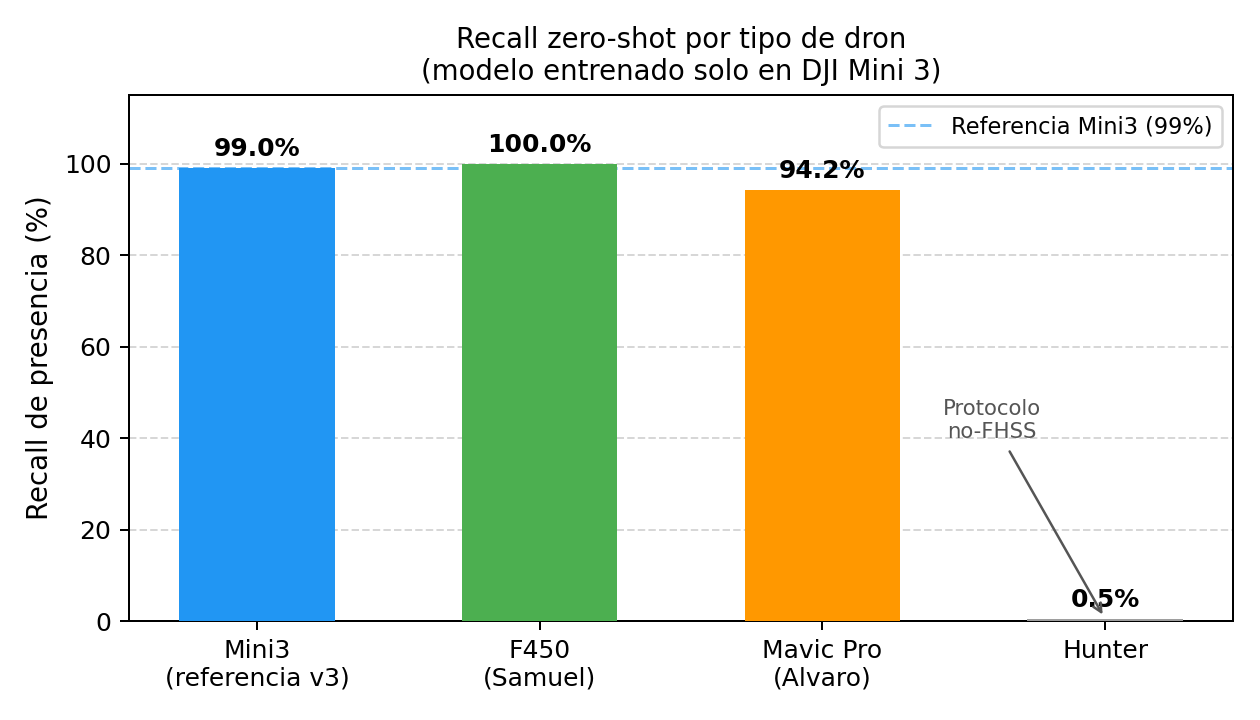
\includegraphics[width=0.8\textwidth]{figuras/resultados/zeroshot_recall_barras.png}
    \caption{Porcentaje de imágenes en las que el detector ---entrenado solo con el Mini~3--- confirma la presencia de dron, para cada plataforma. El F450 y el Mavic~Pro alcanzan el nivel de la referencia del Mini~3; el Hunter se queda en el \SI{0,5}{\percent} por no emitir señal FHSS.}
    \label{fig:zeroshot_recall}
\end{figure}

Los dos drones con protocolo OcuSync~v1 (F450 y Mavic~Pro) se comportan como el Mini~3: detecta en ellos una decena de ráfagas por imagen y confirma su presencia en casi todas las ventanas, sin reentrenamiento y pese a la diferencia de frecuencia. El Hunter, por el contrario, queda prácticamente sin detecciones de dron.

\FloatBarrier
\subsection{Por qué el detector no ve al Hunter}
\label{sec:zeroshot_hunter}

El fallo en el Hunter no es un error del detector, sino la consecuencia esperable de su criterio. El Hunter no transmite mediante saltos de frecuencia: su señal es de espectro ensanchado continuo (compatible con DSSS o un esquema propietario), sin las ráfagas compactas y separadas que caracterizan a OcuSync. Como el detector aprendió a buscar precisamente esa forma ---columnas cortas y aisladas en el plano tiempo-frecuencia--- y el Hunter no la presenta, no encuentra nada que marcar como dron.

Conviene subrayar un matiz: el detector no ignora la señal del Hunter, sino que la \emph{ve} y la clasifica como \emph{interference}. De hecho emite una media de \num{7,5}~cajas de interferencia por espectrograma, con al menos una en la totalidad de las \num{788}~imágenes. Es decir, reconoce que hay una señal activa, pero su morfología no es la de un salto FHSS, así que la asigna a la clase de interferencia y no a la de dron. El Hunter queda, por tanto, fuera del dominio para el que el sistema fue diseñado: el detector está pensado para señales FHSS, y el Hunter no lo es.

Este resultado, lejos de ser un punto débil, es la prueba más clara de qué ha aprendido el modelo. El detector reconoce la morfología FHSS allí donde aparece ---en drones distintos, con protocolos distintos y en frecuencias distintas--- y deja de detectar únicamente cuando esa morfología no existe. No ha memorizado al DJI~Mini~3: ha aprendido a reconocer la huella que deja un salto de frecuencia.

\subsection{Alcance del experimento: capturas de señal limpia}
\label{sec:zeroshot_alcance}

Conviene interpretar estas cifras tan altas en su justo contexto. Las capturas de campo de los tres drones se realizaron, en su mayoría, en condiciones de \emph{señal limpia}: con el dron como emisor dominante, a distancias moderadas y sin inyección de ruido ni interferencia intensa que solapara con sus ráfagas. Este experimento no pretende medir la robustez del detector frente al ruido ---esa cuestión se aborda por separado en el barrido de SNR del experimento P4---, sino responder a una pregunta más concreta: ¿reconoce el detector la morfología FHSS de un dron que nunca ha visto cuando esa morfología es claramente visible en el espectrograma? Para aislar esa pregunta es necesario, precisamente, partir de capturas en las que la firma del dron no esté enmascarada.

Por ello, los recall cercanos al \SI{100}{\percent} del F450 y el Mavic~Pro deben leerse como el rendimiento del detector en condiciones favorables, no como una garantía de comportamiento en cualquier escenario. En un despliegue real ---con interferencia WiFi y Bluetooth densa, mayores distancias, ángulos de antena desfavorables o niveles de señal más bajos--- es esperable que el recall descienda, igual que ocurría en el dataset~v3 del Mini~3 con las capturas más difíciles. El único indicio en esa dirección dentro de este experimento son las dos sesiones del Mavic~Pro con señal débil y las capturas con WiFi denso, donde el rendimiento ya muestra cierta sensibilidad a las condiciones de captura.

En resumen, lo que demuestra este experimento es la \emph{capacidad de transferencia} del detector a drones nuevos cuando la señal es observable, no su robustez en condiciones adversas. Ambas propiedades son necesarias para un sistema de vigilancia completo, pero se validan con experimentos distintos: la transferencia aquí, y la robustez frente al ruido en P4. La validación conjunta ---drones no vistos \emph{y} en condiciones de interferencia controlada--- requiere un conjunto de datos específico y queda planteada como trabajo futuro (dataset~v4).

\section{Discusión global}
\label{sec:discusion}

Las cuatro preguntas anteriores, junto con el experimento de detección de drones no vistos de la \cref{sec:zeroshot}, trazan una evolución metodológica coherente. La primera establece que la firma OcuSync es aprendible por un clasificador global en condición limpia, pero identifica los límites de esa formulación: ausencia de localización, incapacidad para representar clases coexistentes y riesgo de sesgo de contexto en escenarios de despliegue más generales. La segunda demuestra que un detector de objetos supera esas limitaciones localizando morfológicamente las ráfagas con cero confusión cruzada, al precio de un recall de caja moderado que se explica por el etiquetado automático débil y la ligereza del modelo. La tercera muestra que ese recall moderado no impide una vigilancia operativa fiable: agregando varias detecciones por ventana temporal se alcanza el \SI{91}{\percent} de recall de presencia con precisión y especificidad perfectas. La cuarta cierra el argumento con dos resultados complementarios: el clasificador de modelos identifica el DJI Mini~3 sin errores, y el barrido de robustez demuestra cuantitativamente que la discriminación se basa en la morfología y no en la intensidad. Este experimento confirma esa hipótesis desde fuera del conjunto de entrenamiento: el detector generaliza a OcuSync~v1 (F450 y Mavic~Pro) sin reentrenamiento, clasifica activamente la señal del Hunter como interferencia ---demostrando que ve la señal pero distingue su morfología de la FHSS--- y mantiene robustez frente a cambios de frecuencia central de hasta \SI{50}{\mega\hertz}.

El principal resultado positivo del sistema es la ausencia de falsos positivos en todas las condiciones evaluadas: cuando el detector afirma que una ráfaga es de dron, no se equivoca de clase; y cuando el clasificador de presencia confirma que hay un dron en la escena, no se equivoca de imagen. La principal limitación es el recall a nivel de caja, consecuencia del etiquetado automático ruidoso, el reducido tamaño de las ráfagas tras el redimensionado y el uso de un modelo ligero. El análisis de presencia demuestra que esta limitación es tolerable en condición operativa; sin embargo, mejorar el etiquetado ---ya sea con datos adicionales o con anotación manual parcial de las ráfagas más débiles--- es la vía más directa para aumentar la sensibilidad del sistema.

Operativamente, el sesgo del sistema hacia falsos negativos (no detectar una ráfaga individual) es preferible al sesgo hacia falsos positivos (confirmar presencia de dron en una escena sin dron), especialmente en un contexto de primera alerta donde una alarma espuria tiene coste operativo. El sistema en dos etapas se comporta como una primera versión sólida de vigilancia RF, cuyo margen de mejora reside en la cobertura de ráfagas individuales y no en la separabilidad entre clases.
